\documentclass[10pt]{article}

%% Various useful packages and commands from different sources

\usepackage[applemac]{inputenc}
\usepackage[english]{babel}
\usepackage[T1]{fontenc}
\usepackage{cite, url,color} % Citation numbers being automatically sorted and properly "compressed/ranged".
%\usepackage{pgfplots}
\usepackage{graphics,amsfonts}
\usepackage[pdftex]{graphicx}
\usepackage[cmex10]{amsmath}
% Also, note that the amsmath package sets \interdisplaylinepenalty to 10000
% thus preventing page breaks from occurring within multiline equations. Use:
 \interdisplaylinepenalty=2500
% after loading amsmath to restore such page breaks as IEEEtran.cls normally does.

% Compact lists
\usepackage{enumitem}
\usepackage{booktabs}
\usepackage{fancyvrb}

\usepackage{listings} % for Matlab code
\definecolor{commenti}{rgb}{0.13,0.55,0.13}
\definecolor{stringhe}{rgb}{0.63,0.125,0.94}
\lstloadlanguages{Matlab}
\lstset{% general command to set parameter(s)
framexleftmargin=0mm,
frame=single,
keywordstyle = \color{blue},% blue keywords
identifierstyle =, % nothing happens
commentstyle = \color{commenti}, % comments
stringstyle = \ttfamily \color{stringhe}, % typewriter type for strings
showstringspaces = false, % no special string spaces
emph = {for, if, then, else, end},
emphstyle = \color{blue},
firstnumber = 1,
numbers =right, %  show number_line
numberstyle = \tiny, % style of number_line
stepnumber = 5, % one number_line after stepnumber
numbersep = 5pt,
language = {Matlab},
extendedchars = true,
breaklines = true,
breakautoindent = true,
breakindent = 30pt,
basicstyle=\footnotesize\ttfamily
}

\usepackage{array}
% http://www.ctan.org/tex-archive/macros/latex/required/tools/
\usepackage{mdwmath}
\usepackage{mdwtab}
%mdwtab.sty	-- A complete ground-up rewrite of LaTeX's `tabular' and  `array' environments.  Has lots of advantages over
%		   the standard version, and over the version in `array.sty'.
% *** SUBFIGURE PACKAGES ***
\usepackage[tight,footnotesize]{subfigure}
\usepackage[top=2cm, bottom=2cm, right=1.6cm,left=1.6cm]{geometry}
\usepackage{indentfirst}


\setlength\parindent{0pt}
\linespread{1}

\usepackage{mathtools}
\DeclarePairedDelimiter{\ceil}{\lceil}{\rceil}
\DeclarePairedDelimiter{\floor}{\lfloor}{\rfloor}
\DeclareMathOperator*{\argmax}{arg\,max}


% equations are numbered section by section
\numberwithin{equation}{section}


\begin{document}
\title{Digital Transmission - Homework 1}
\author{Andrea Dittadi, Davide Magrin, Michele Polese}

\maketitle

\section*{Introduction}
This report is organized as follows: as first the spectral analysis of the process is presented, along with our considerations on the position of the spectral lines. Then we will describe the filter used to separate the spectral lines and the continuous part from the original signal, and their AR models. Then LMS and RLS algorithms and their implementation will be discussed. In the last section there is the description of a method that computes frequency, amplitude and phase of the spectral lines.

\section{Estimating the PSD}
% some lines on what is PSD?
In order to estimate the PSD of a given a process $z(k)$ it is necessary to consider two hypotheses. The first is that the process is at least wide sense stationary. A process $z(k)$ is WSS if $m_z(t) = m_z, \forall t$ and $r_z(t, t - \tau) = r_z(\tau), \forall t$. By inspecting the mean and autocorrelation over different non-overlapping windows of 100 samples it appears that the mean is quite constant, as is the estimate of the real part of the autocorrelation, while the imaginary part of the autocorrelation changes more than the two other estimates. Instead, by considering the sample mean of different subsequences of 20 samples inside each bigger window the real and imaginary parts of the mean don't vary too much, despite the great variance that an estimator with few samples has. We conclude that in each window of less than 100 sample the process can be considered WSS, while it is harder to state that it is WSS in all the 1000 samples.
% Because of this consideration we will use windows of 100 samples to analyze the PSD of the process and derive conclusions on the presence of the spectral lines.

% Do we agree on this Does it make sense? Can we provide some figures?
% Or we skip these considerations and say that it is wss?

The second hypothesis is that the process is ergodic, and as suggested in \cite{bc} we assume that every WSS process is also ergodic. In this way from a single representation of the process it is possible to estimate the autocorrelation and thus the PSD of the whole process. This is a key assumption for the analysis of the process we are given, without this hypothesis not much can be said. \\
We also subtract the sample mean $\hat{\mu}_z = \frac{1}{K} \sum_{i=1}^K z(k)$ by the given signal $z(k)$, since the deterministic component doesn't bring any relevant information to the estimates of the PSD of the process. Thus the signal to which we will refer in the following spectral analysis is a zero-mean signal with the form $z(k) = z(k) - \hat{\mu}_z$ with $K$ the number of samples of the signal. \\
In order to estimate the PSD of the process and find the spectral lines we used a combination different estimators that will be introduced in the following sections. \\
Note that unless specified we assume a unitary sampling period $T_c = 1$.

\subsection{Unbiased estimate of autocorrelation}
\label{sec:unbauto}
The autocorrelation is estimated using
\begin{equation}
  \hat{r}_z(n) = \frac{1}{K - n}\sum_{k=n}^{K-1} z(k) z^*(k-n)
  \label{eq:auto}
\end{equation}
with $n = 0, 1, ... K/5$ in order to avoid poor estimates given by the fact that, as $n$ approaches $K$, the number of samples used in the estimate becomes smaller and smaller, and the variance of the estimator increases.

\subsection{Periodogram}
The periodogram is an estimator of the PSD based on the Fourier transform of the signal:
\begin{equation}
  \mathcal{P}_{PER} = \frac{1}{K T_c} |\mathcal{\tilde{Z}}(f)|^2
\end{equation}
The Fourier transform $|\mathcal{\tilde{Z}}(f)|$ is computed as a DTFT with the function \verb fft  provided in MATLAB. This is a biased estimator, because of the fact that the signal is windowed over a finite number of samples. In order to improve the quality of this estimate and to detect more precisely the spectral lines it is possible to apply another window, instead of the rectangular one. In particular, in some cases we applied a Kaiser window (from \cite{mitra}) to the signal before the computation of the \verb fft. This is a tunable window in the form of
\begin{equation}
  w(k) = \frac{I_0 \bigg[w_a \sqrt{1-\big(1-\frac{2(n+1)}{L+1}\big)^2}\bigg]}{I_0[w_a]} \; \; \; \; \; \;  0 \le n < L
\end{equation}
where $I_0[x]$ is the zero-order Bessel function and $w_a$ is a tunable parameter that depends on the attenuation of the secondary lobes of the window. In this way it is possible to reduce spectral leakage and make real spectral lines stand out among the peaks produced by the noise. For an attenuation $A_{dB} > 50$ dB then $w_a = 0.1102(A_{dB} - 8.7)$. Given the length and the parameter $w_a$, the Kaiser window can be computed using MATLAB function \verb kaiser .
% Alternatively, $w_a = 5.65$ -> 60 dB %

\subsection{Welch periodogram}
The idea behind the Welch periodogram is to compute the periodograms on different windows of the given signal and to average them for each frequency. Each subsequence $z^{(s)}$ is composed of $D$ consecutive samples of the original signal, and has $S$ samples in common with the previous and the following windows. Thus given the length $K$ of the original signal the number of subsequences is $N_s = \floor{\frac{K - D}{D - S} + 1}$. For each subsequence $z^{(s)} = w(k)z(k + s(D-S)), \; k=0,1,..., D- 1, \; s = 0, 1, ... N_s - 1$, with $w(k)$ a window of $D$ samples and normalized energy $M_w = \frac{1}{D}\sum_{k=0}^{D-1}w^2(k)$, we compute the periodogram $\mathcal{P}_{PER}^{(s)}(f) = \frac{1}{D T_c M_w} |\mathcal{\tilde{Z}}^{(s)}(f)|^2$.
Therefore the Welch estimate is given by
\begin{equation}
  \mathcal{P}_{WE}(f) = \frac{1}{N_s}\sum_{s=0}^{N_s-1}{P}_{PER}^{(s)}(f)
\end{equation}


\subsection{Blackman and Tukey correlogram}
This estimator uses an unbiased autocorrelation sequence estimate ${\hat{r}_z(n)}, n = -L, ..., L$ as specified in Section~\ref{sec:unbauto}. It computes the Fourier transform of the ACS multiplied by a window $w(k)$ of length $2L + 1$ and $w(0)=1$ (both requirements are satisfied by the Kaiser window of the previous section):
\begin{equation}
  \mathcal{P}_{CORR}(f) = T_c\sum_{n=-L}^{L}w(n)\hat{r}_z(n)e^{-j2\pi f n T_c}
\end{equation}
Note that $L \le K/5$ because of the considerations about the variance of ACS estimate. In particular we chose $L = K/5$. Moreover the ACS estimator of Equation~\ref{eq:auto} is computed for non-negative values of $n$, so the samples for $n =-1, -2, ..., -L$ are computed exploiting the hermitian symmetry of the ACS ($\hat{r}_z(-n) = \hat{r}_z^*(n)$). \\

\subsection{AR model}
\label{sec:ar}
The last estimate of the PSD can be computed using an AR model of order N to describe the process. This model considers the process as generated by a recursive equation
\begin{equation}
  z(k) = - \sum_{n=1}^N a_n z(k-n) + w(k)
\end{equation}
with $w$ white noise with variance $\sigma_w^2$. This equation is equivalent to a scheme where $w$ is filtered by a filter with transfer function $H_{AR}(z) = 1/A(z)$ with $A(z) = 1 + \sum_{n=1}^N a_n z^{-n}$. Then the z-transform of the ACS is given by $P_z(z) = \frac{\sigma_w^2}{A(z)A^*(\frac{1}{z^*})}$, therefore the PSD, which is the Fourier transform of the ACS, is
\begin{equation}
  \mathcal{P}_{AR} = P_z(e^{j 2 \pi f T_c}) = \frac{\sigma_w^2}{|\mathcal{A}(e^{j 2 \pi f T_c})|^2} = \frac{\sigma_w^2}{|\mathcal{A}(f)|^2}
  \label{eq:arpsd}
\end{equation}
The coefficients $a_1, a_2, ..., a_N$ can be computed using the Yule-Walker equations. Given the autocorrelation matrix
\begin{equation}
  \mathbf{R} =
  \begin{bmatrix}
     r_z(0) &  r_z(-1) & \cdots &  r_z(-N+1) \\
     r_z(1) &  r_z(0)  & \cdots &  r_z(-N+2) \\
    \vdots       & \vdots        & \vdots & \vdots \\
     r_z(N-1) &  r_z(N-2) & \cdots &  r_z(0)
  \end{bmatrix}
\end{equation}
and $ \mathbf{r} = [r_z(1),  r_z(2),  r_z(N)]^T $ the vector $\mathbf{a}$ of the coefficients of the AR model is given by
\begin{equation}
  \mathbf{R} \, \mathbf{a} = - \mathbf{r}
  \label{eq:yw}
\end{equation}
and the variance of the white noise driving the model is
\begin{equation}
  \sigma_w^2 = \hat{r}_z(0) + \mathbf{r}^H\mathbf{a}
\end{equation}
Since the complete statistical description of the process isn't available, we compute the autocorrelation matrix $\mathbf{R}$ using a biased ACS estimate as suggested in \cite{bc}. The biased estimate of autocorrelation differs from the unbiased one in Equation~\ref{eq:auto} by the normalization factor which is set to the length of the signal $K, \; \; \forall n$. Therefore $\mathbf{R}_{(i, j)} = \check{r}_z(i - j)$, where the samples for $n = i - j=-1, -2, ..., -N$ are estimated using the hermitian symmetry of the ACS. \\


\subsection{Identification of spectral lines}
The identification of spectral lines is usually carried out by inspection of the PSD of the process. In this problem there are two factors that make this procedure unfeasible: the low signal to noise ratio and the small number of samples we are given. Moreover the hypothesis of wide sense stationarity should be considered carefully, since we don't know the nature of the underlying process. \\
The low amplitude of the spectral lines, compared to the power of the noise, doesn't allow to clearly distinguish their presence by inspecting the PSD estimated in different ways over the whole 1000 samples. There are some peaks but it isn't straightforward to conclude that they represent noise peaks or spectral lines. On the other side, there's some literature on detection of sinusoidal components with low amplitude in wideband noise, such as the article in \cite{lowamp}, but the proposed algorithms require more than 1000 samples.\\
This behavior can be seen in Figure~\ref{fig:complete_psd} where different estimates of the PSD are plotted.
\begin{figure}[htp]
  \centering
  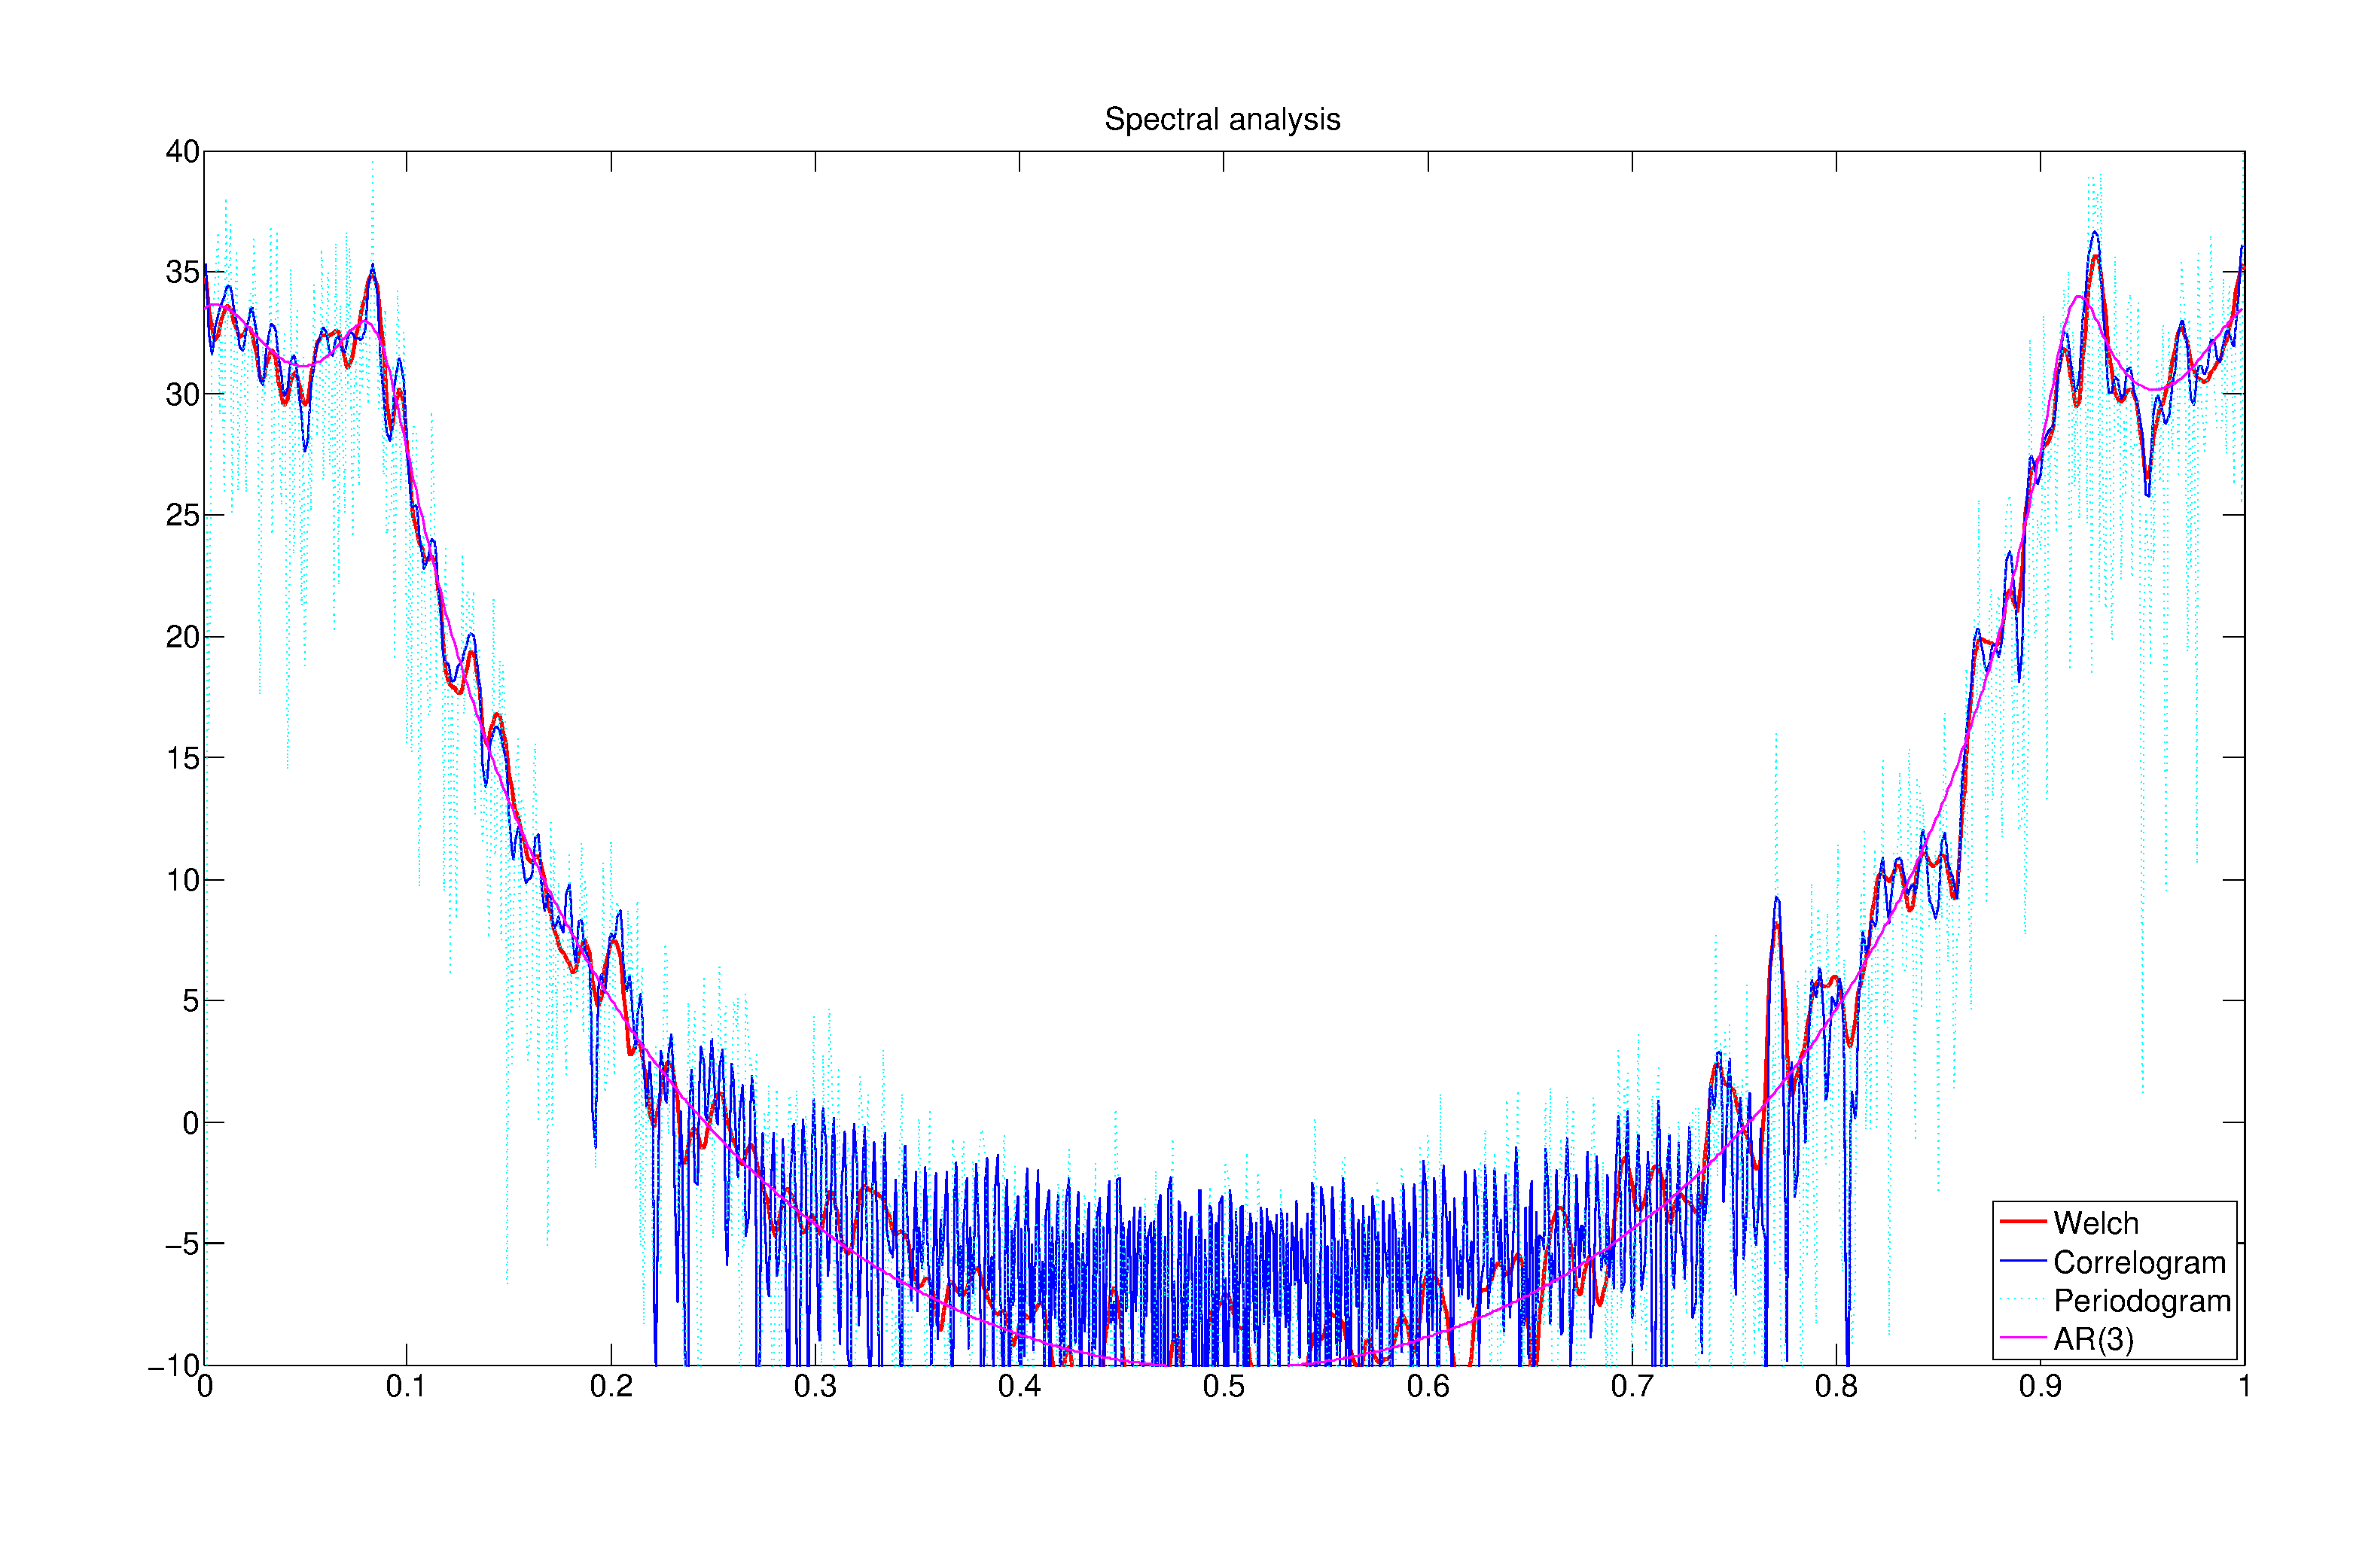
\includegraphics[width=0.9\textwidth]{images/psd}
  \caption{Different spectral estimates}
  \label{fig:complete_psd}
\end{figure}
The parameters of the estimators are as follows. For the periodogram the window used is the default rectangular one. For Welch periodogram $D = 200$, $S = D/2$ and the window chosen is a Kaiser window with sidelobe attenuation of 60 dB ($w_a = 5.65$). The order of the autocorrelation estimator for the correlogram is $N_{corr} = K/5 = 200$, the window applied is once again a Kaiser window with 60 dB sidelobe attenuation. The AR model has order 3, since the knee of the noise variance $\sigma_w^2$ is present at $N=3$ as it can be seen in Figure~\ref{fig:complete_knee}.

\begin{figure}
  \centering
  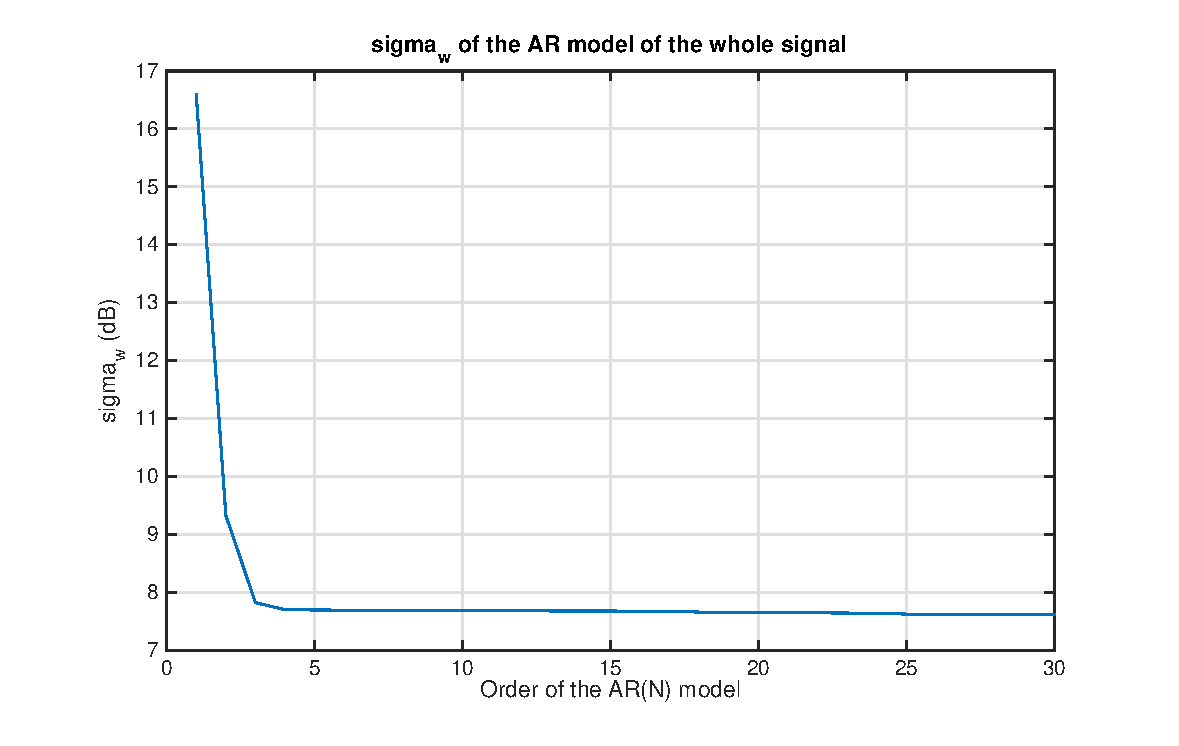
\includegraphics[width = 0.7\textwidth]{images/complete_knee}
  \caption{Variance of AR model white noise as a function of the order N}
  \label{fig:complete_knee}
\end{figure}

In order to identify which peaks in Figure~\ref{fig:complete_psd} belong to the noise and which are given by low amplitude spectral lines we developed an algorithm that tries to tackle the issues described before and produce some clear results. At first it considers different windows of samples, of length $L$ and with the initial samples separated by $S$ samples. They overlap by $\max\{0, L-S\}$ samples. The number of windows is $N = \floor{(K-L)/S}$ with $K$ the length of the whole signal. For each of these short windows the algorithm computes the periodogram and finds its peaks (defined as local maxima, the algorithm uses the function \verb findpeaks  of MATLAB). It keeps a running sum of the peaks found at each frequency (note: they are quantized by the length $L$ of the window chosen, and the eventual zero padding of the fft) and increases its value by 1 whenever there's a peak. In this way it artificially observes more than one realization of the process: if a peak in the periodogram is due to the noise present at a certain instant it could be absent in the next windows. On the other hand, if a peak is due to a weak sinusoidal signal it will be present in more than one window and the sum of peaks found at that frequency will be higher than the number of peaks at frequencies with just the noise. We chose to consider the periodogram and not the other estimators because the length $L$ of the windows we considered is always below or equal 100 samples, otherwise the number of different windows $N$ would be too low. The Welch and correlogram estimator are less effective with so few samples. For the first there's a necessary trade-off between the number of windows $N_s$ and their length $D$: the number of samples in each window should be enough to represent the process, but the smaller $N_s$ is the more the Welch periodogram becomes similar to a simple periodogram, with high variance. Also the Blackman and Tukey correlogram suffers in the presence of short windows because it transforms the estimate of the ACS, which is reliable only if computed on less than a fifth of the window's samples.\\
\begin{figure}[htp]
  \centering
  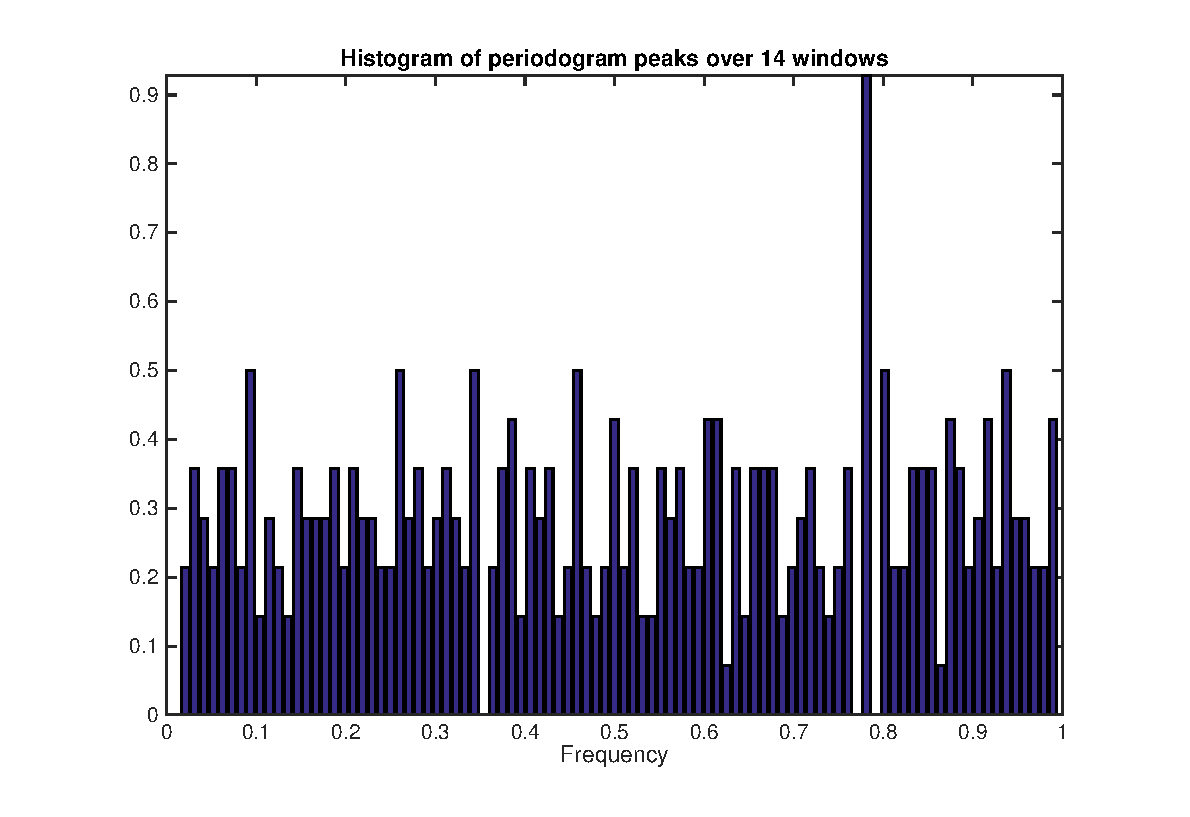
\includegraphics[width = 0.7\textwidth]{images/period_acc}
  \caption{Accumulation of peaks in the signal}
  \label{fig:peak_acc}
\end{figure}

In Figure~\ref{fig:peak_acc} there's the result of an iteration of the algorithm on the given signal, with parameters $S = 64$, $L = 96$ and a periodogram computed by windowing the signal with a Kaiser window with parameter $w_a = 5.65$ which guarantees a sidelobe attenuation of 60 dB, without increasing the size of the main lobe too much (this allows us to reduce spectral leakage without increasing the smearing too much).

In can be clearly seen that there is a peak for $f_0 = 0.77$ in about 90\% of the windows, while the other peaks are much lower. Thus we conclude that the only spectral line present in the signal has the form $A e^{j 2 \pi f_0 n T_c}$. This peak is present also in Figure~\ref{fig:complete_psd} and periodogram, Welch and correlogram represent it. The AR model, instead, doesn't change its behavior in the presence of the peak, probably because the amplitude of the complex sinusoid is too low.

There are a couple other methods we designed in order to determine the presence of spectral lines. One involves a whitening filter: as it can be seen from the PSD estimates, the signal has a lowpass behavior. This can interfere with the identification of the spectral lines: if one is located in the middle frequency range, its power will be several dBs below the higher power frequencies, that can be nonetheless caused by noise. Because of this, an equalization of the PSD has been attempted, in order to neutralize the higher power of the lower frequencies of the signal. Because this attempt was only driven by the desire to locate precisely spectral lines, we neglect phase considerations at this stage.

To equalize the spectrum, the periodogram estimate of the signal has been multiplied by the inverse of the frequency response of the filter given by the AR model. This is equal to the use of a whitening filter: if the signal is thought of as the result of white noise filtering (for which the filter has the same coeffients yielded by the AR model), the inverse of this filter will bring every frequency more or less at the same power. In this situation, it is easier to identify spectral lines, as they could clearly emerge from the white noise, now reduced to a constant. In fact, after passing the signal through such a whitening filter, it can be seen that its representation in the frequency domain is that in Figure~\ref{fig:whitening}. At the $0.77 F_c$ frequency there is a peak that is 5 dB above the rest of the white noise. This can be interpreted as a strong indication of the presence of a spectral line.


\section{AR models for continuous and spectral lines components}
In order to separate the spectral line from the whole signal we used the cascade of two filters, that is their convolution in the time domain. A simple passband filter centered at $f_0 = 0.77$ is not enough because the PSD at that frequency is 20 dB below the PSD at frequencies $f \in [0, 0.1]$ and $f \in [0.9, 1]$. Therefore the signal is as first filtered with a real FIR linear-frequency highpass filter that equalizes the PSD and then with a complex FIR linear-frequency bandpass filter centered at $f_0 = 0.77$.

The complex bandpass filter is designed using MATLAB function \verb cfirpm , which uses the Remez exchange algorithm adapted to the complex case. The filter has a linear phase, its transition bands are $[f_0 - 0.02, f_0 - 0.002]$ and $[f_0 + 0.002, f_0 + 0.02]$. The real highpass filter is designed with MATLAB \verb firpm  called in \verb fdatool  by using the Parks-McClellan algorithm (based on Remez exchange too).

Actually the filtering is done in one step with a filter which is the convolution of the two ($h_{lines}(k) = (h_{hp}*h_{bp})(k)$), thus the transfer function will be $H_{lines}(z) = H_{bp}(z)H_{hp}(z)$. The order of the filter is $N = 76$, thus the delay is $D = N/2 = 38$ samples. Then the continuous part is isolated by the original signal using a filter which is the complementary of the previous one, which is $H_{continuous}(z)= 1 - H_{lines}(z)$. Note that since the filter has to be causal, the constant factor 1 has to be multiplied by the factor $e^{j*\frac{N}{2}}$, therefore in the time domain the analog transformation is $h_{continuous}(k) = \delta(k - \frac{N}{2}) - h_{lines}(k)$. \\
Note that filtering is performed on the provided signal $z(k)$. \\
The frequency and phase response of the filters used is in Figures~\ref{fig:line_filt} and~\ref{fig:cont_filt}.\\

\begin{figure}[h!]
  \centering
  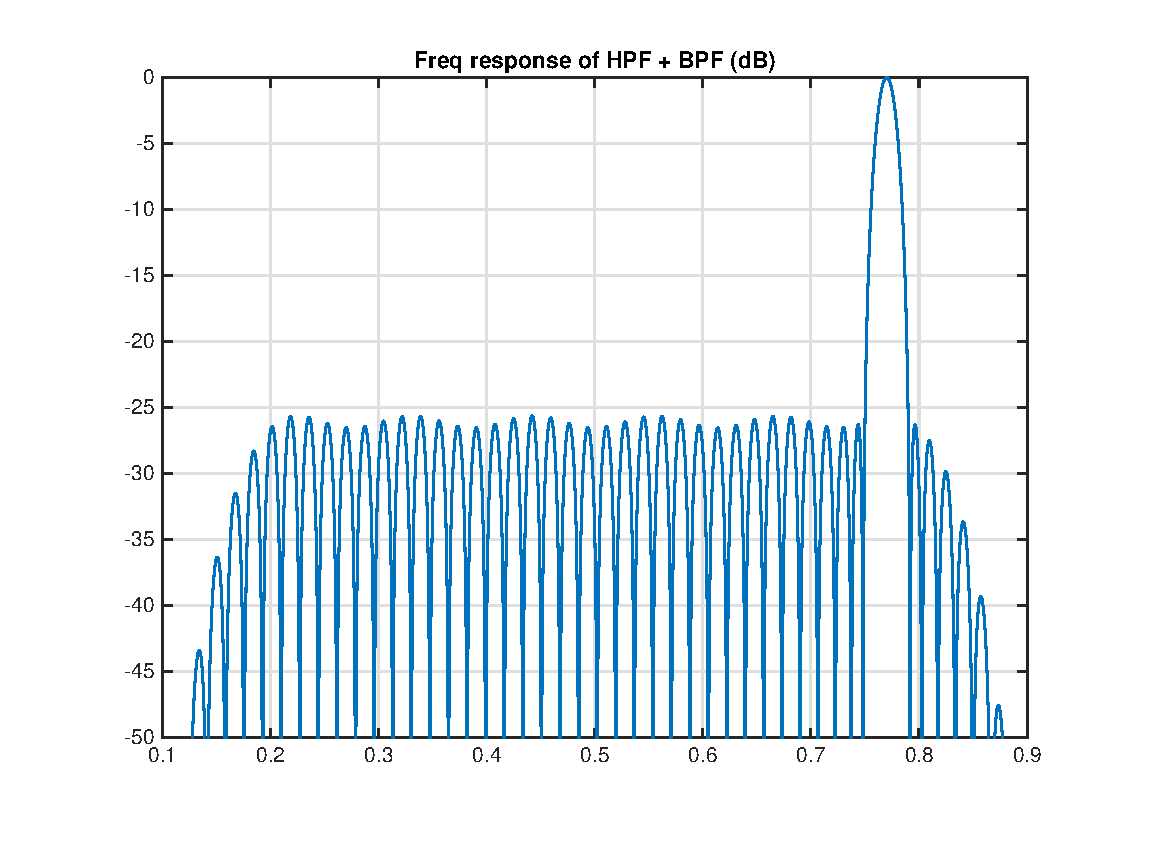
\includegraphics[width = 0.7\textwidth]{images/filter_lines}
  \caption{Frequency response of spectral lines filter $h_{lines}$}
  \label{fig:line_filt}
\end{figure}

\begin{figure}[h!]
  \centering
  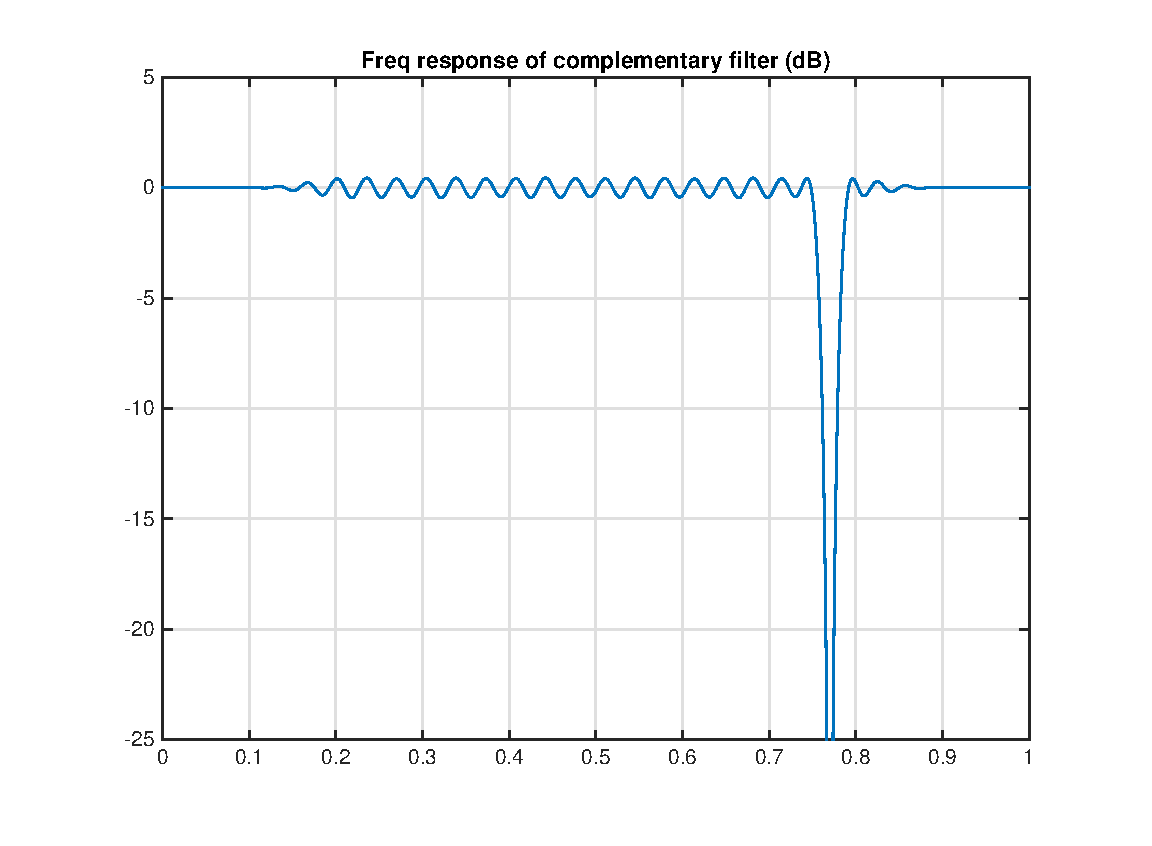
\includegraphics[width = 0.7\textwidth]{images/filter_continuous}
  \caption{Frequency response of filter $h_{continuous}$ for the continuous PSD}
  \label{fig:cont_filt}
\end{figure}

With these filters the maximum of the difference between the original signal, delayed by the transient $D$, and the sum of the continuous part and the spectral line part of the signal is $5.685 \times 10^{-14}$. \\

\subsection*{AR model for the continuous-PSD signal}
The continuous-PSD signal $z_{\text{continuous}}$ is then analyzed with the AR model proposed in Section~\ref{sec:ar}. In Figure~\ref{fig:ar_cont_sigma} there is the plot of the variance $\sigma_w^2$ of the white noise which feeds the model as a function of the order $N$, and it can be seen that the knee is at $N=3$. % Comments?
Therefore the order of the AR model is $N=3$. The vector of coefficients that solves the Yule-Walker Equation~\ref{eq:yw} is $\mathbf{a} = [-2,
.37 - j0.012, 2.071 + j0.023, -0.65 - j0.015]^T$ thus $A(z) = 1 + \sum_{i=1}^3a_i z^{-i}$, and the variance of the noise $\sigma_w^2 = 6.2887$ dB. \\ %(only linear or only dB?)
In Figure~\ref{fig:zpl_cont} there's the plot of zeros of $A(z)$ in the complex plane, while Figure~\ref{fig:psd_cont} reports the AR(3) estimate of the PSD computed with Equation~\ref{eq:arpsd}.

% plots from filter_fir.m section on AR model of continuous part
\begin{figure}[h!]
  \centering
  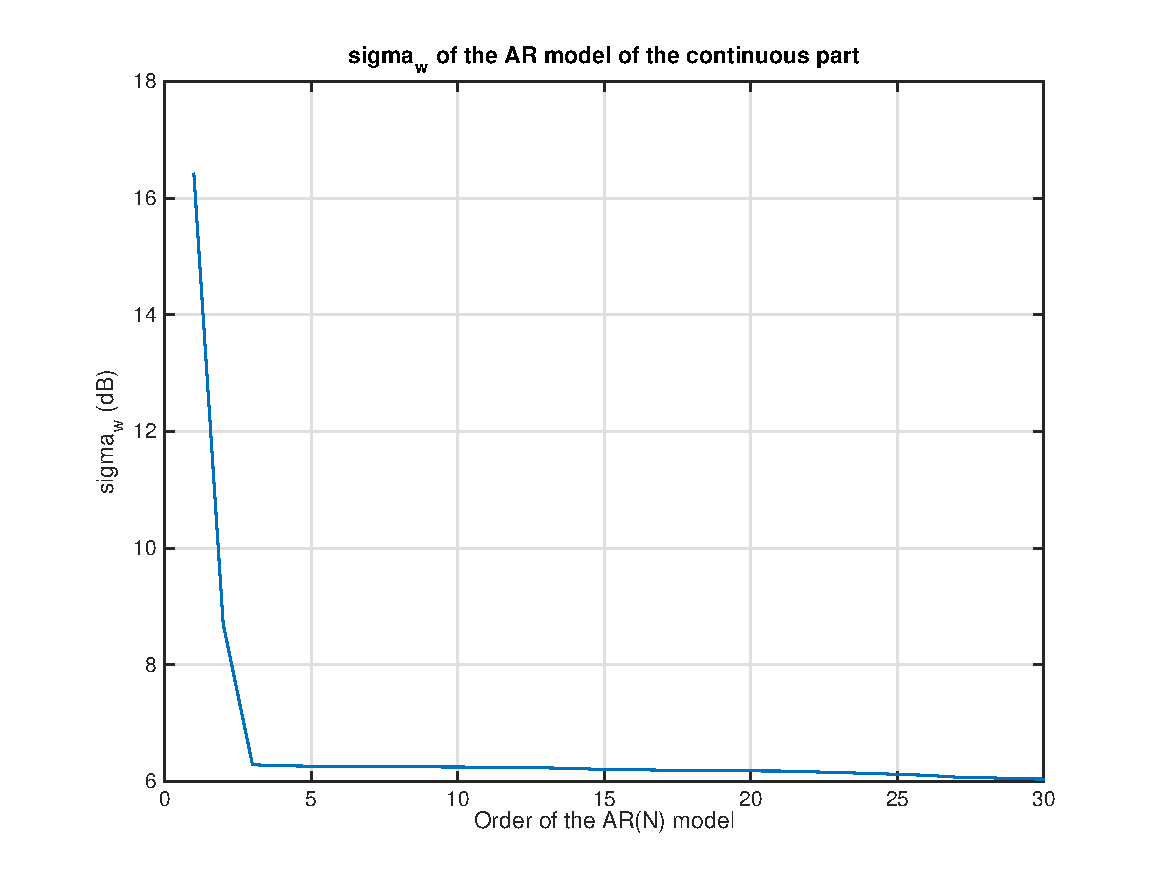
\includegraphics[width = 0.7\textwidth]{images/ar_continuous_sigma}
  \caption{AR model for continuous-PSD signal: variance $\sigma_w^2$ of the noise as a function of N}
  \label{fig:ar_cont_sigma}
\end{figure}

\begin{figure}[h!]
  \centering
  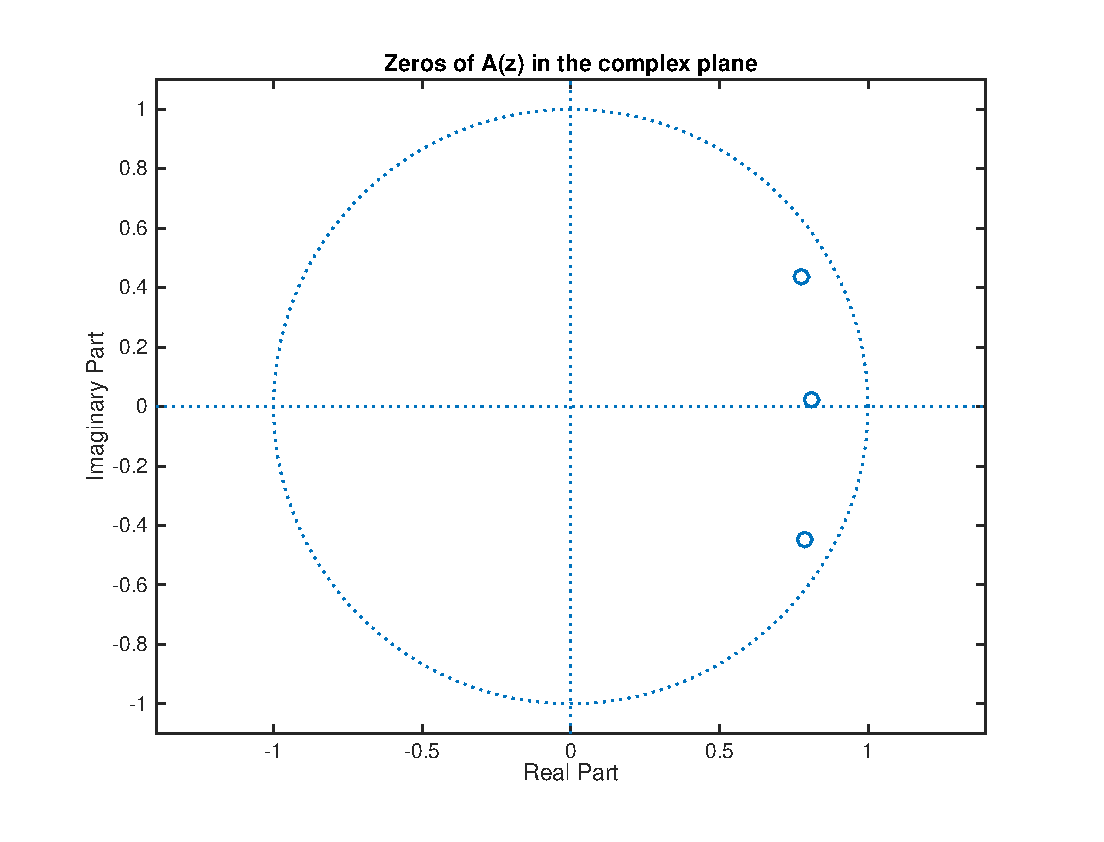
\includegraphics[width = 0.7\textwidth]{images/ar_continuous_zeros}
  \caption{AR model for continuous-PSD signal: zeros of $A(z)$ in the complex plane}
  \label{fig:zpl_cont}
\end{figure}

\begin{figure}[h!]
  \centering
  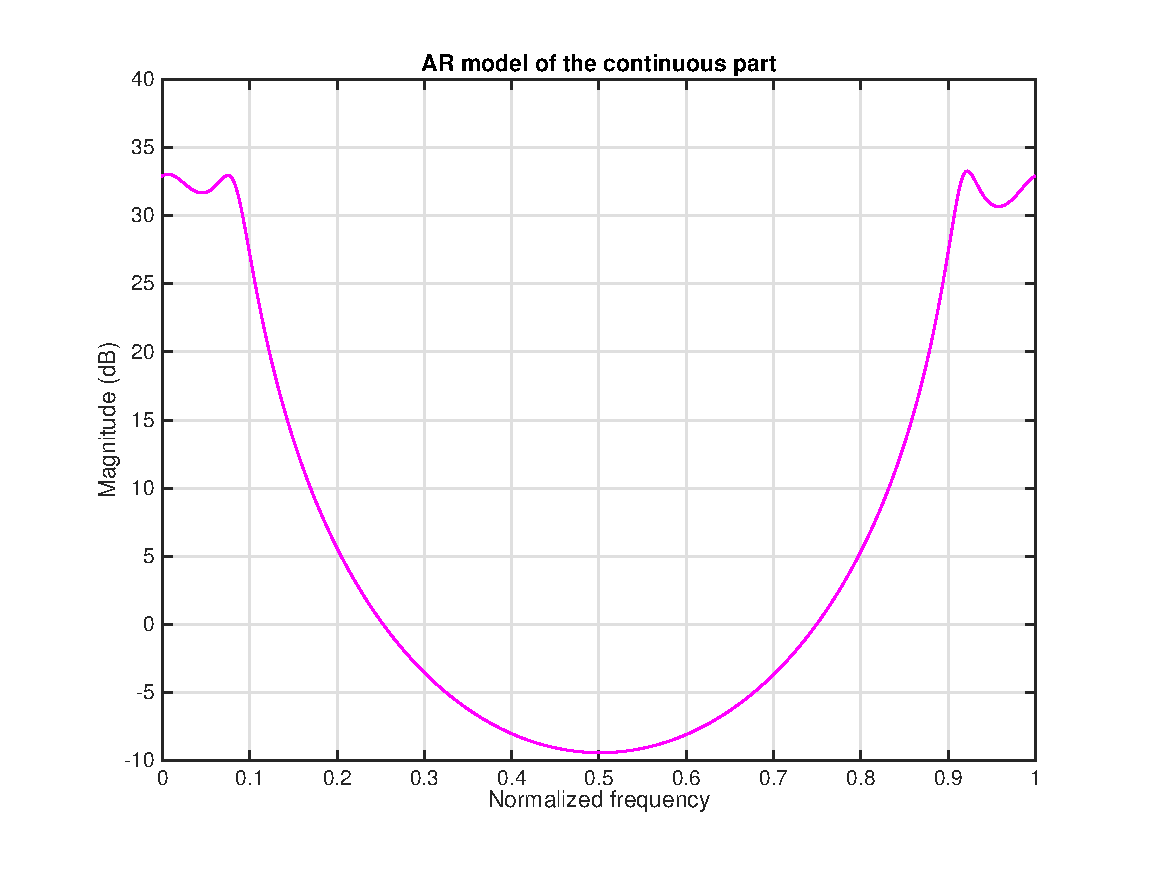
\includegraphics[width = 0.7\textwidth]{images/ar_continuous_psd}
  \caption{AR model for continuous-PSD signal: AR(3) estimate of the PSD of continuous-PSD signal}
  \label{fig:psd_cont}
\end{figure}


\subsection*{AR model for the spectral lines}
Also the signal with the spectral line $z_{\text{lines}}$ is analyzed with an AR model.
In Figure~\ref{fig:ar_lines_sigma} there is the plot of the variance $\sigma_w^2$ of the white noise versus the order $N$, and it can be seen that the knee is at $N=5$. Actually there's a first knee also for $N=2$. It must be said that an AR model, in presence of spectral lines, has some poles (zeros of $A(z)$) which are very close to the unit circle, and this could create some numerical problems when it comes to solve the Yule-Walker Equations~\ref{eq:yw}. Moreover an order $N=1$ would be enough to describe a single spectral line, but since the filtering operation is not ideal there is some noise left and an higher order is required to give a better estimate of the actual PSD of $z_{\text{lines}}$.
Therefore let the order of the AR model be $N=5$. The vector of coefficients that solves the Yule-Walker Equation~\ref{eq:yw} is $\mathbf{a} = [-0.0299 + j0.329, 0.985 + j0,023, 0.413 + j0.0959, 0.291 + j0.079, 0.243 + j0.097]^T$ and once again $A(z) = 1 + \sum_{i=1}^5a_i z^{-i}$. The variance of the noise is $\sigma_w^2 = -32.548$ dB. \\ %(only linear or only dB?)
In Figure~\ref{fig:zpl_lines} there's the plot of zeros of $A(z)$ in the complex plane, while Figure~\ref{fig:psd_lines} reports the AR(5) estimate of the PSD computed with Equation~\ref{eq:arpsd}. Note that since the magnitude of the PSD of the spectral line is below 15 dB the scale used for the Y axis in Figure~\ref{fig:psd_lines} has the same dynamic range as Figure~\ref{fig:psd_cont} but it is scaled down of 25 dB.


% plots from filter_fir.m section on AR model of lines part
\begin{figure}[h!]
  \centering
  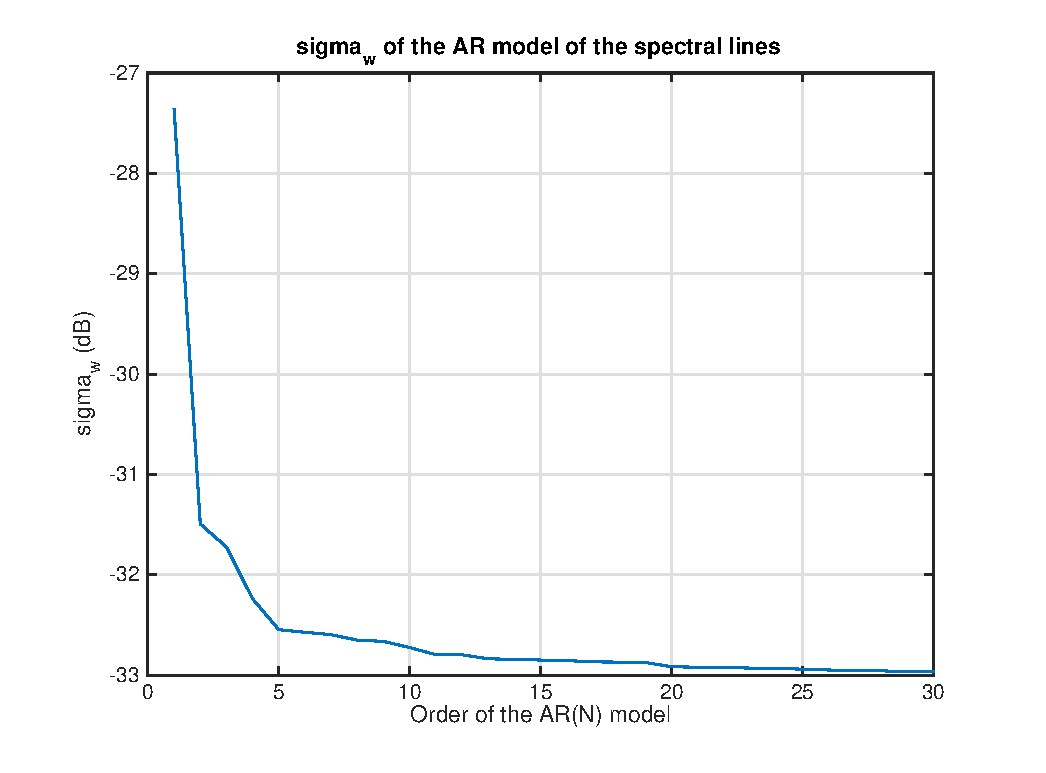
\includegraphics[width = 0.7\textwidth]{images/ar_lines_sigma}
  \caption{AR model for spectral line signal: variance $\sigma_w^2$ of the noise as a function of N}
  \label{fig:ar_lines_sigma}
\end{figure}

\begin{figure}[h!]
  \centering
  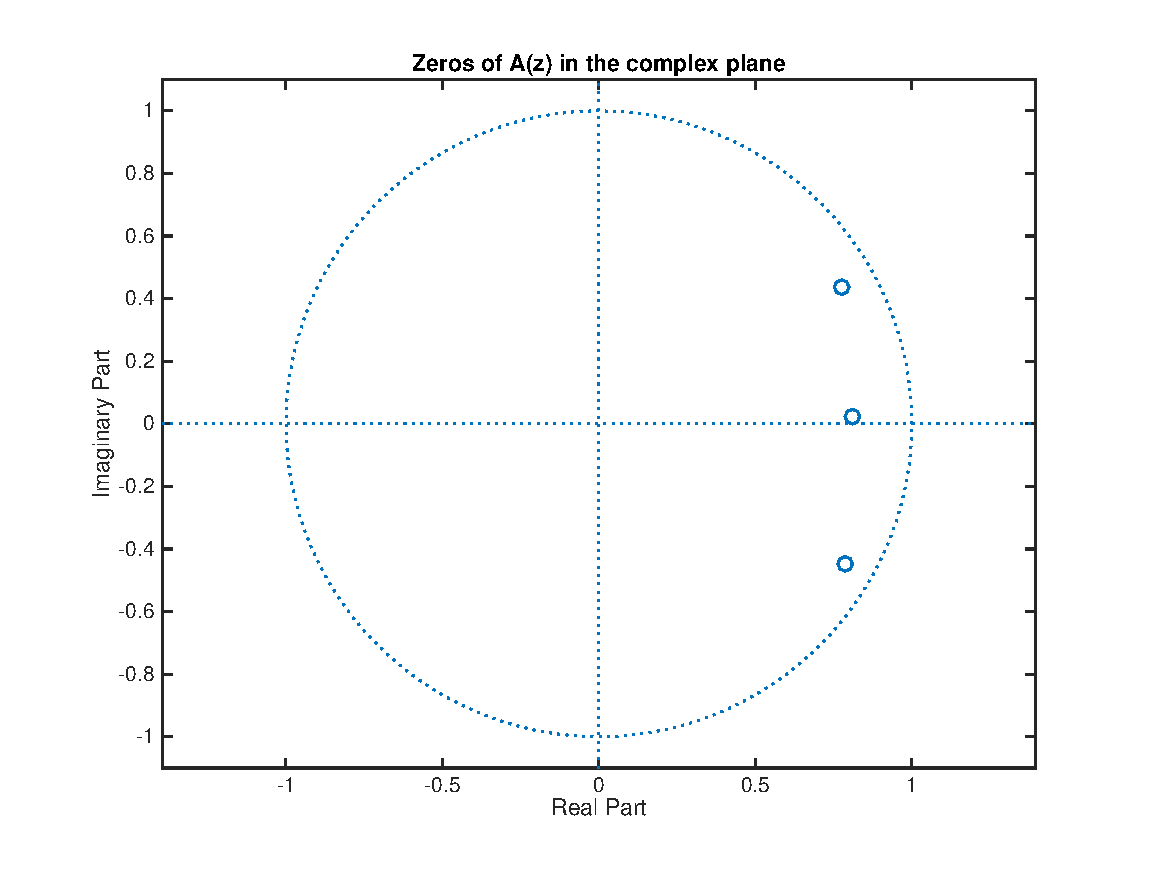
\includegraphics[width = 0.7\textwidth]{images/ar_lines_zeros}
  \caption{AR model for spectral line signal: zeros of $A(z)$ in the complex plane}
  \label{fig:zpl_lines}
\end{figure}


\begin{figure}[htp]
  \centering
  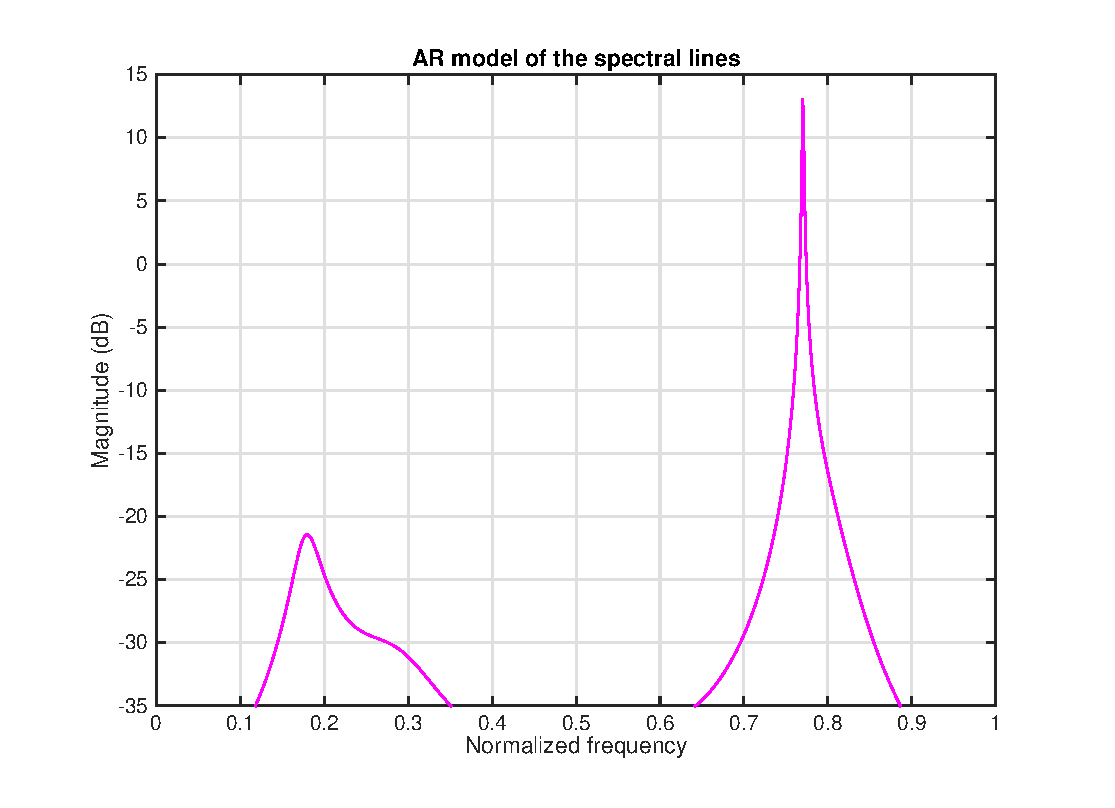
\includegraphics[width = 0.7\textwidth]{images/ar_lines_psd}
  \caption{AR model for spectral line signal: AR(5) estimate of the PSD of spectral line signal}
  \label{fig:psd_lines}
\end{figure}


\section{LMS predictor}
\label{sec:lms}
The setting of the predictor problem is as follows. Given a signal $z(k)$, WSS, with zero mean, let $\mathbf{z}^T(k-1)$ be the vector $[z(k-1), z(k-2), ..., z(k-N)]$. The one-step predictor of order N tries to estimate the value of $z(k)$ given $\mathbf{z}^T(k-1)$. This problem can be solved considering $\mathbf{z}^T(k-1)$ the input of a Wiener filter of order N and $z(k)$ the reference signal. Then the Wiener-Hopf equation computes the optimal coefficients of the filter with
\begin{equation}
  \mathbf{R}_N \mathbf{c}_{opt} = \mathbf{r}_N
  \label{eq:wh}
\end{equation}
given the autocorrelation matrix $\mathbf{R}_N$ and $\mathbf{r}_N = [r_z(1), r_z(2), ..., r_z(N)]^T$. \\
Both \textit{least mean-square} (LMS) and \textit{recursive least square} (RLS) algorithms provide a recursive method to compute an approximation of the optimal Wiener-Hopf solution for the predictor problem without using the autocorrelation matrix $\mathbf{R}_N$ and the vector $\mathbf{r}_N$.
In particular LMS is a version of the gradient algorithm that updates at each iteration $k$ the coefficients of the Wiener filter with the equation
\begin{equation}
  \mathbf{c}(k+1) = \mathbf{c}(k) + \mu e(k) \mathbf{x}^*(k-1)
  \label{eq:lms_up}
\end{equation}
The implementation of LMS is simple and it doesn't require too much computation. There are two parameters, the order $N$ and the update coefficient $\mu = \frac{\tilde{\mu}}{N r_z(0)}$, and it must hold $0 < \tilde{\mu} < 2$ for convergency. Then, at each step, compute:
\begin{equation}
  y(k) = \mathbf{z}^T(k-1) \mathbf{c}(k)
\end{equation}
\begin{equation}
  e(k) = z(k) - y(k)
\end{equation}
and update coefficients with Equation~\ref{eq:lms_up}. At the beginning $\mathbf{c}(0) = \mathbf{0}$, and $z(k) = 0, \; \forall \; k < 0$. \\
We tested our implementation of LMS against a known process, generated using an AR model of order $N = 3$ with coefficients $\mathbf{a} = [1, 0.2-0.5i, 0.2, 0.2]$ and white noise variance $\sigma_w^2 = 0$ dB. The length of the generated signal is $K = 5000$ samples, enough to ensure convergence also with a low $\tilde{\mu}$ (actually $\tilde{\mu} = 0.01$), that we chose in order to have a small error. Then $\mathbf{c_{opt}} = -\mathbf{a}$, with $\mathbf{c_{opt}}$ the optimum coefficients  of the Wiener-Hopf equation and $\mathbf{a}$ the solution of the Yule-Walker equation for the AR model, and $\sigma_w^2 = J_N$, with $J_N$ the cost function of the Wiener filter approximated by $|e(k)|^2$ in the LMS algorithm. Therefore the coefficients $\mathbf{c}$ and the $|e(k)|^2$ of the LMS algorithm should converge in mean to $-\mathbf{a}$ and $\sigma_w^2$ respectively.
In order to test if this behavior holds, we simulate 500 times the process and apply in each iteration the LMS algorithm. In this way it is possible to estimate the mean of the coefficients $\mathbf{c}$ and of the error square $|e(k)|^2$. The results are in Figures~\ref{fig:coeff_lms_test} and~\ref{fig:err_lms_test} and it can be seen that the algorithm converges in the mean to the red horinzontal lines which represent the values of $-\mathbf{a}$ and $\sigma_w^2$.

% plots from lms_test.m
\begin{figure}[h!]
\centering
	\subfigure{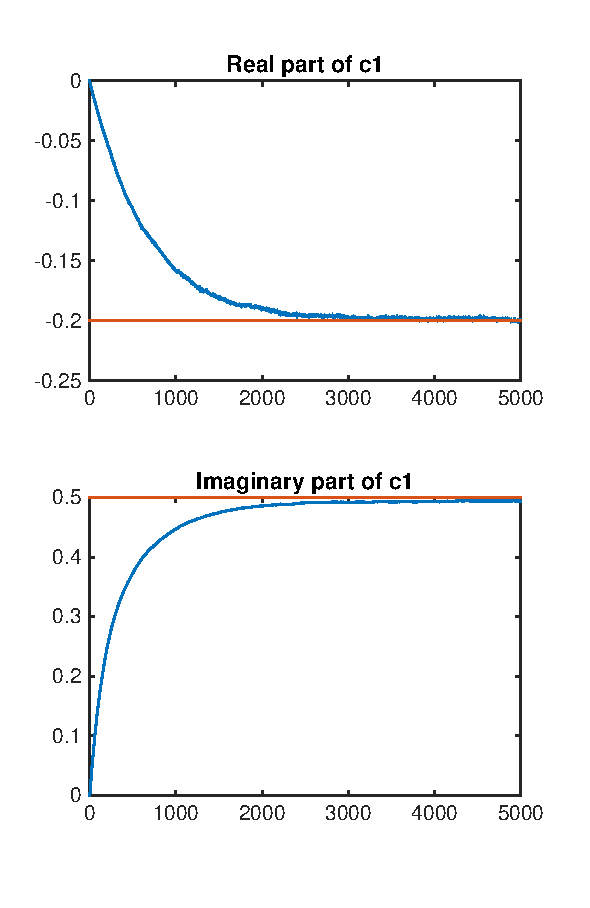
\includegraphics[width=0.3\textwidth]{images/lmstest_c1}}
	\subfigure{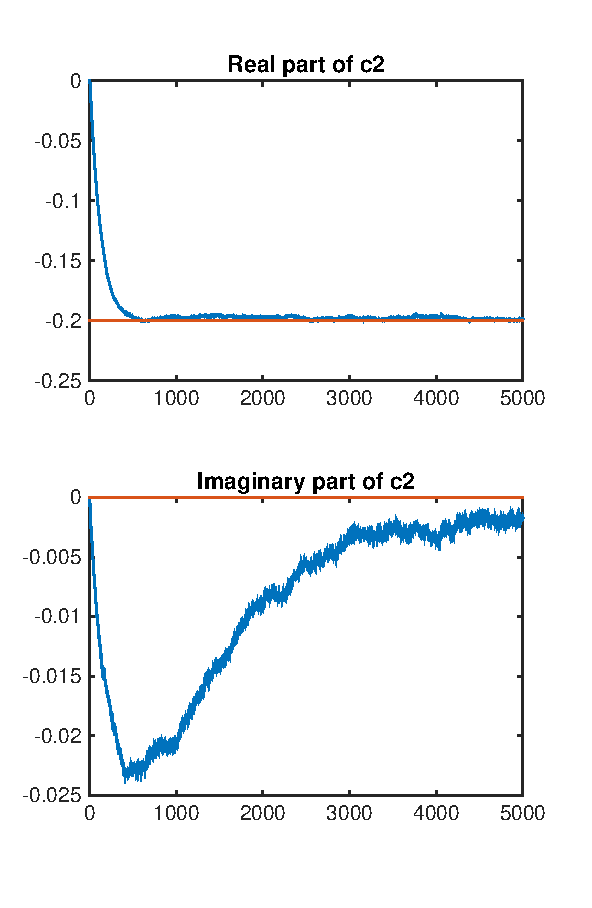
\includegraphics[width=0.3\textwidth]{images/lmstest_c2}}
	\subfigure{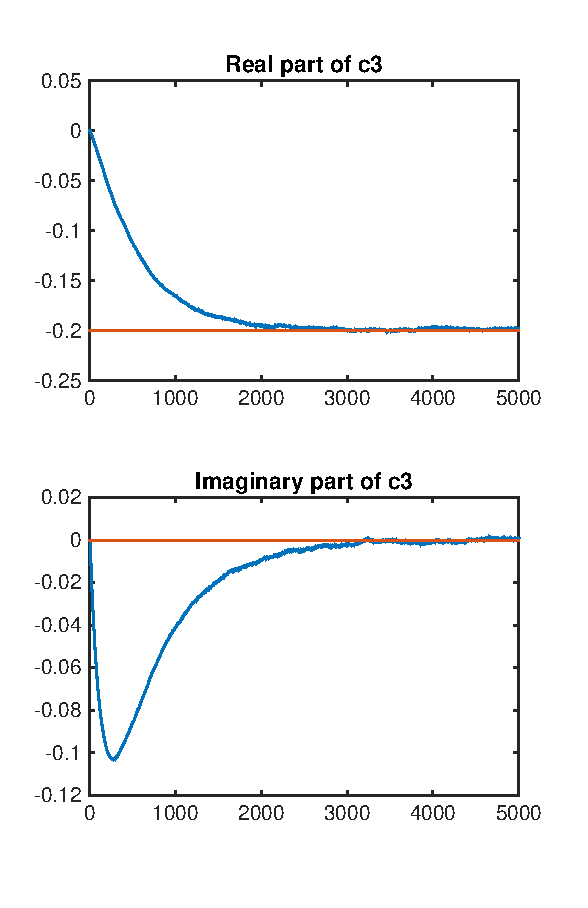
\includegraphics[width=0.3\textwidth]{images/lmstest_c3}}
 	 \caption{Average of coefficients $\mathbf{c}$ (real and imaginary part) over 500 simulations}
  \label{fig:coeff_lms_test}
\end{figure}

\begin{figure}[h!]
  \centering
  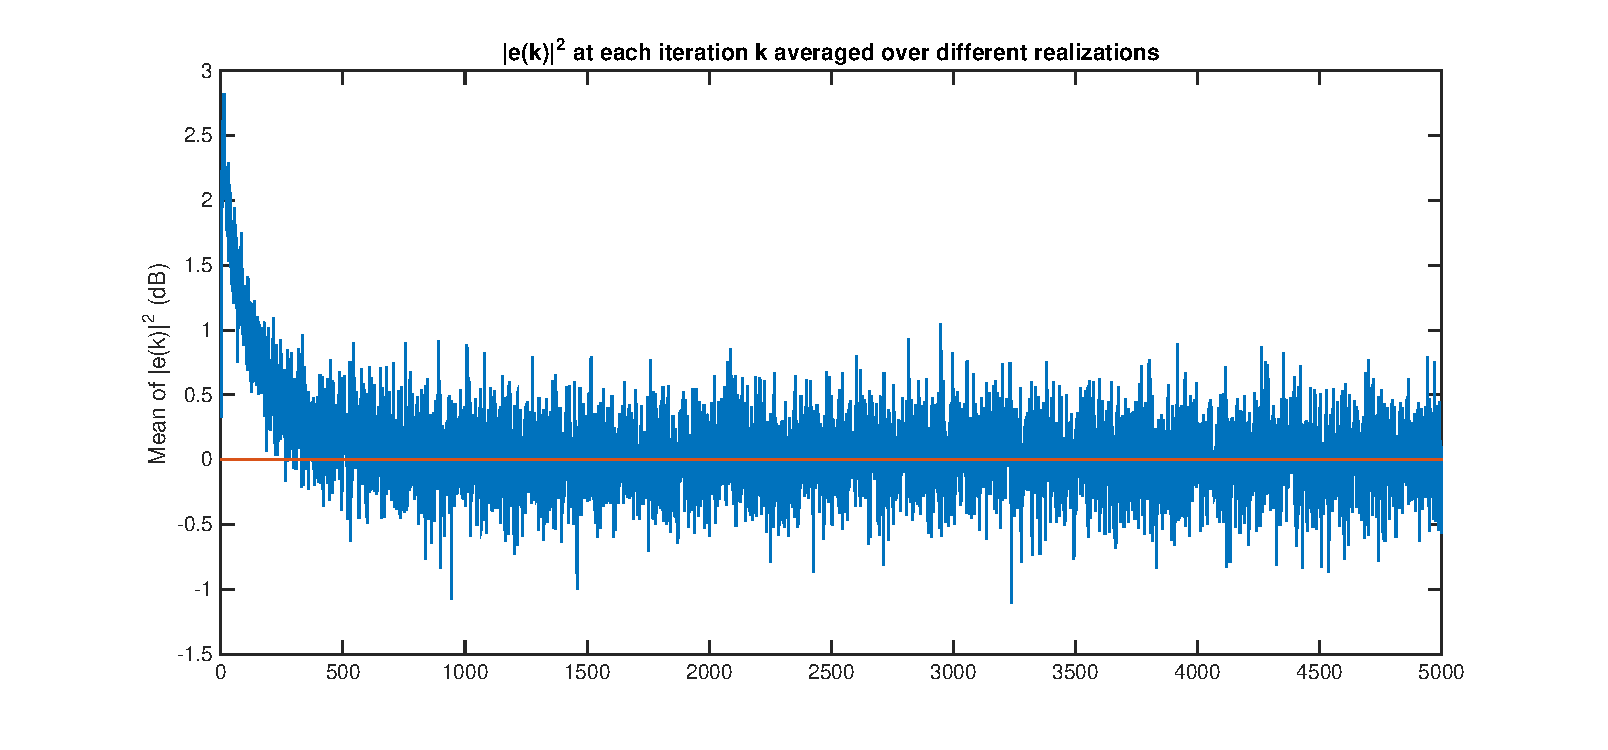
\includegraphics[width = 0.7\textwidth]{images/lmstest_err}
  \caption{Average of $|e(k)|^2$ over 500 simulations}
  \label{fig:err_lms_test}
\end{figure}


Then we applied the LMS algorithm to the continuous part of the signal as filtered in Section 2. Given the AR model of order N = 2 for the continuous part of the signal, the $\mathbf{c}$ vector should converge to $-\mathbf{a}$ and $|e(k)|^2 = \sigma_w^2$ at least in mean. This can be seen in Figures~\ref{fig:coeff_lms} and~\ref{fig:err_lms}

%plots from lms.m
\begin{figure}[h!]
	\centering
	\subfigure{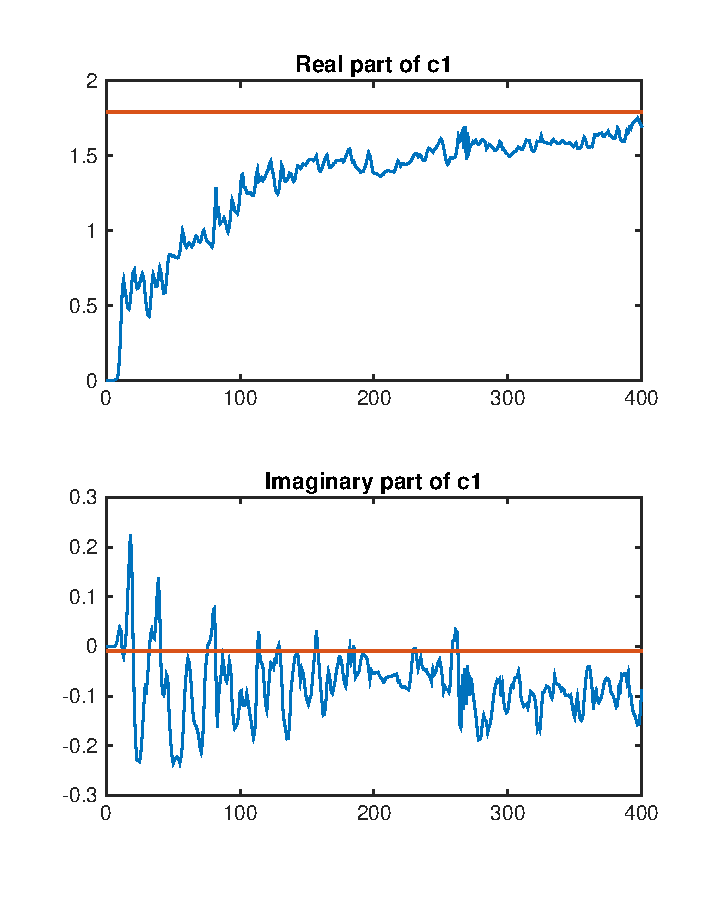
\includegraphics[width=0.48\textwidth]{images/lms_c1}}
	\subfigure{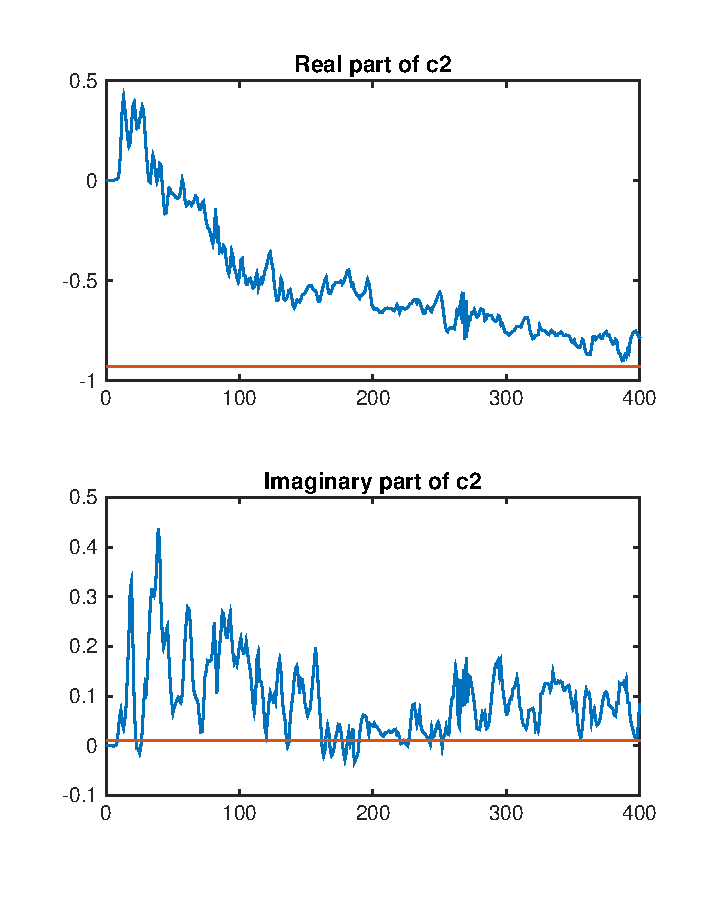
\includegraphics[width=0.48\textwidth]{images/lms_c2}}
  \caption{Coefficients $\mathbf{c}$ (real and imaginary part) over 400 iterations of LMS}
  \label{fig:coeff_lms}
\end{figure}

\begin{figure}[h!]
  \centering
  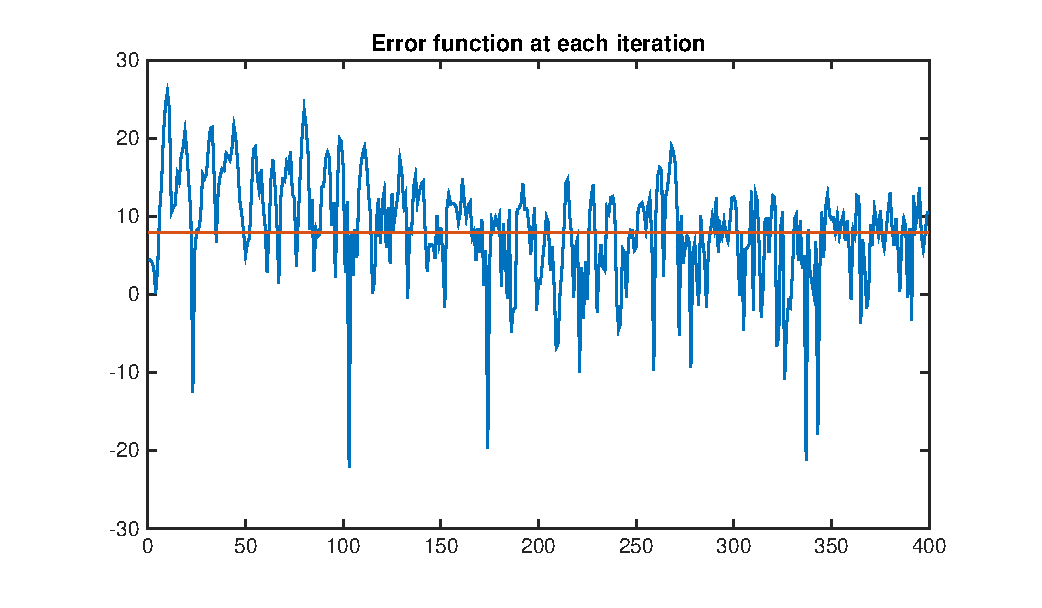
\includegraphics[width = 0.7\textwidth]{images/lms_err}
  \caption{$|e(k)|^2$ over 400 iterations of LMS}
  \label{fig:err_lms}
\end{figure}

Note that the algorithm is applied on only one realization of the process and this is the reason of the grassy behavior of the coefficients and the error: we observe just one realization and not the average other many. The value of $\tilde{\mu} = 0.42$ ensures the convergence in the 400 iterations required. The value of coefficients at iteration $k = 350$ and the average of $|e(k)|^2$ over the window $k \in [350 - 10, 350 + 10]$ can be found in Table~\ref{table:lms_conv}. A lower value for $\tilde{\mu}$ would have generated a smaller error at convergency but in 400 iterations it wouldn't have reached it, thus the values in Table~\ref{table:lms_conv} would have been farther from the ones they should converge to ($-\mathbf{a}$ and $|e(k)|^2 = \sigma_w^2$).
\begin{table}[h!]
  \centering
  \begin{tabular}{c|c|c}
    $c_1(350)$ &   $c_2(350)$ & $\frac{1}{21}\sum_{k=340}^{360} |e(k)|^2$ [dB] \\ \hline
    $1.5738 - j0.1428$ & $-0.8088 + j0.0744$ & $8.365$
  \end{tabular}
  \caption{Values of coefficients and $|e(k)|^2$ of LMS at $k=350$}
  \label{table:lms_conv}
\end{table}

\section{RLS algorithm}
The setting for the RLS predictor is the same as described in Section~\ref{sec:lms}. It is an algorithm that provides a recursive solution for the Wiener-Hopf Equation~\ref{eq:wh} as like as LMS, but it has a faster convergency at the cost of a larger computational complexity. \\
Let $\mathbf{c}^T(k) = [c_1(k), c_2(k), ..., c_N(k)]$ the vector of $N$ coefficients at instant $k$, $\mathbf{z}^T(i) = [z(i-1), z(i-2), ..., z(i-N)]$ the input of the filter at instant $i$ and $y(i) = \mathbf{c}^T(k)\mathbf{z}(i) = \mathbf{z}^T(i)\mathbf{c}(k)$ the output of the filter at instant $i$ obtained with coefficients at instant $k$. Since this is a predictor the reference signal $d(i) = z(i)$, the error at each iteration is $e(k) = z(k) - y(k)$. Finally let $\lambda$ be a forgetting factor.\\
The algorithm is quite complex, it begins with an initialization phase. The vector of coefficients at instant $0$ is $\mathbf{c}(0) = \mathbf{0}$ and the auxiliary matrix $\mathbf{P}(k)$ is $\mathbf{P}(0) = \frac{100}{\hat{r}_x(0)} \mathbf{I}$ with $\mathbf{I}$ the identity matrix of size $N\times N$. Then at each iteration $k = 1, 2, ...$:
\begin{equation}
  \mathbf{\Pi}^*(k) = \mathbf{P}(k-1)\mathbf{z}^*(k)
\end{equation}
\begin{equation}
  r(k) = \frac{1}{\lambda + \mathbf{z}^T(k)\mathbf{\Pi}^*(k)}
\end{equation}
\begin{equation}
  \mathbf{k}^*(k) = r(k)\mathbf{\Pi}^*(k)
\end{equation}
\begin{equation}
  \epsilon(k) = z(k) - \mathbf{z}^T(k)\mathbf{c}(k-1)
\end{equation}
\begin{equation}
  \mathbf{c}(k) = \mathbf{c}(k-1) + \epsilon(k)\mathbf{k}^*(k)
\end{equation}
\begin{equation}
  \mathbf{P}(k) = \lambda^{-1}(\mathbf{P}(k-1) - \mathbf{k}^*(k)\mathbf{\Pi}^T(k))
\end{equation}
with $\mathbf{\Pi}, \mathbf{k}, \epsilon(k), r(k)$ auxiliary entities that allow a lower computational complexity. Moreover, since it is required to compute the cost function $\mathcal{E}(k) = \sum_{i=1}^k \lambda^{k-i} |e(i)|^2$ for each iteration, compute also
\begin{equation}
  \mathcal{E}_{min}(k) = \lambda \mathcal{E}_{min}(k-1) + \epsilon(k)e^*(k)
\end{equation}
In our implementation $\lambda = 1$. \\
The convergence of this algorithm is actually faster than the one of LMS algorithm. Since the underlying problem is the same as for LMS, given the AR model of order $N$ of the process, also in RLS algorithm the $\mathbf{c}$ vector should converge to $-\mathbf{a}$ and $\mathcal{E}_{min}(k) = \sigma_w^2$ at least in mean. Since we apply the algorithm to just one realization of the process the average behavior cannot be observed, but as it can be seen in Figures~\ref{fig:rls_coeff} and~\ref{fig:err_rls} the convergence is reached in few iterations also in this single realization.

%plots from rls.m
\begin{figure}[h!]
\centering
	\subfigure{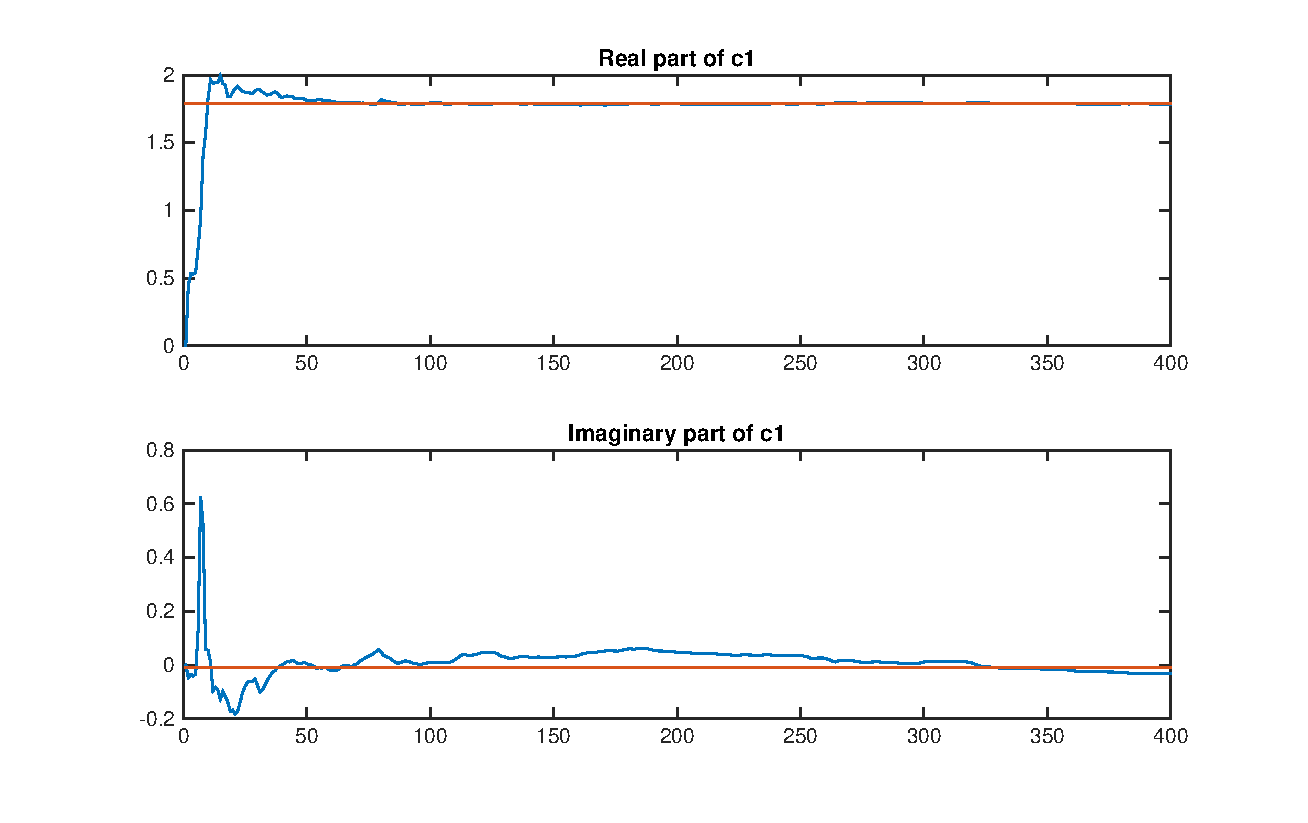
\includegraphics[width=0.75\textwidth]{images/rls_c1}}

	\subfigure{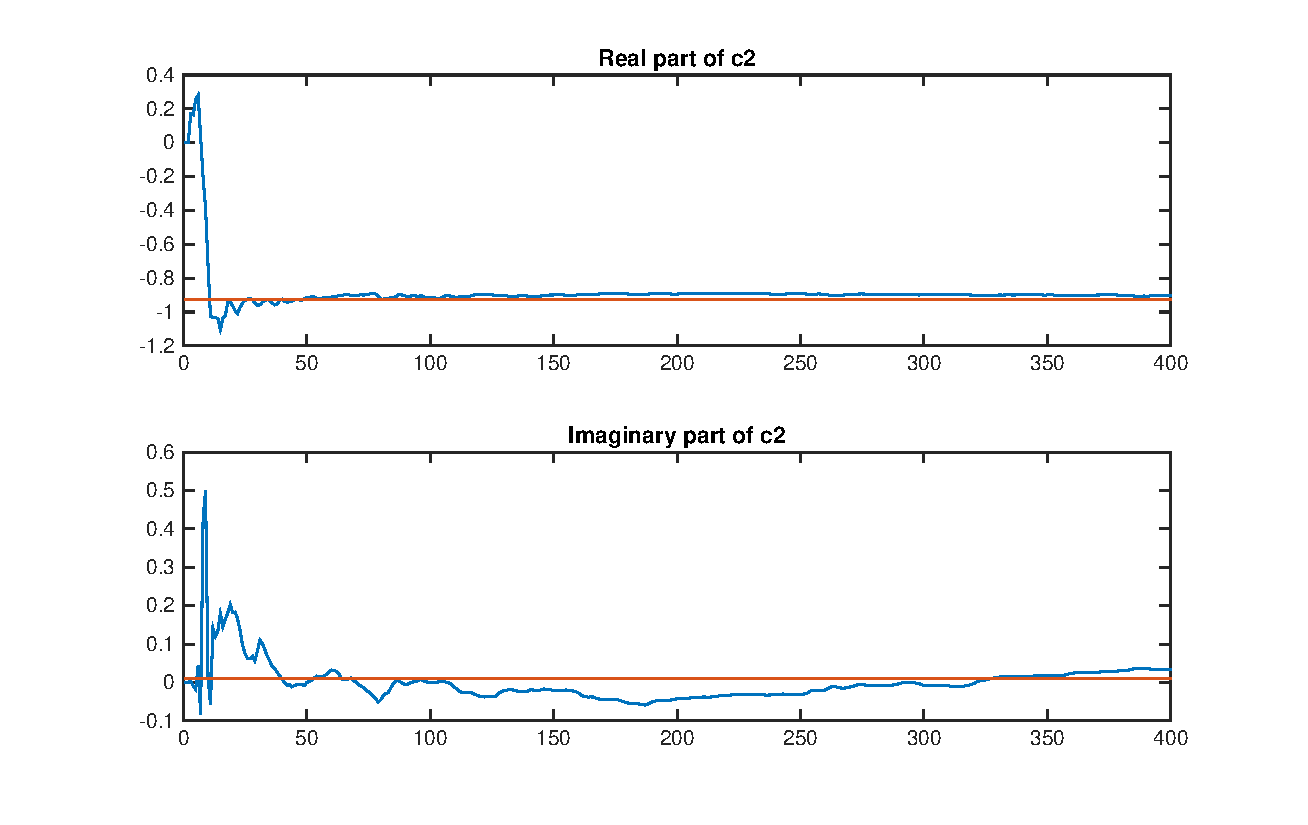
\includegraphics[width=0.75\textwidth]{images/rls_c2}}
  \caption{Coefficients $\mathbf{c}$ (real and imaginary part) over 400 iterations of RLS}
  \label{fig:rls_coeff}
\end{figure}

\begin{figure}[h!]
  \centering
  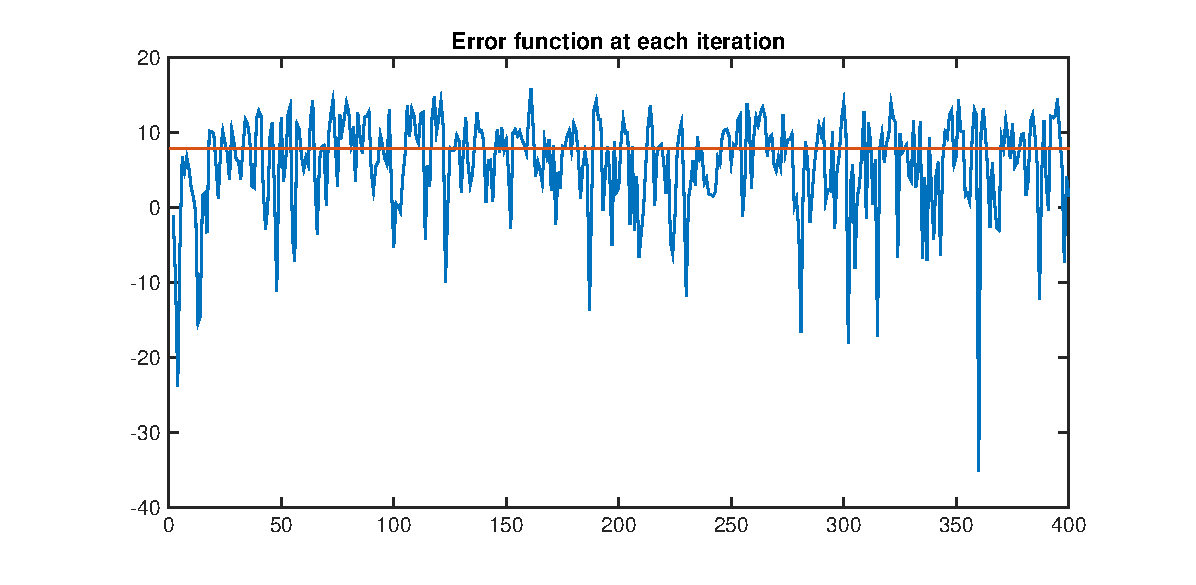
\includegraphics[width = 0.7\textwidth]{images/rls_err}
  \caption{$\mathcal{E}_{min}(k)$ over 400 iterations of RLS}
  \label{fig:err_rls}
\end{figure}

The value of coefficients at iteration $k = 350$ and the average of $\mathcal{E}_{min}(k)$ over the window $k \in [350 - 10, 350 + 10]$ can be found in Table~\ref{table:rls_conv}. It can be seen, both from Figures~\ref{fig:rls_coeff} and~\ref{fig:err_rls} and Table~\ref{table:rls_conv} that the coefficients are closer to the value they should converge to, while the functional $\mathcal{E}_{min}(350)$ has a larger value.

\begin{table}[h!]
  \centering
  \begin{tabular}{c|c|c}
    $c_1(350)$ &   $c_2(350)$ & $\frac{1}{21}\sum_{k=340}^{360} \mathcal{E}_{min}(k)$ [dB] \\ \hline
    $1.789 - j0.0148$ & $-0.899 + j0.0177$ & $9.6372$
  \end{tabular}
  \caption{Values of coefficients and $\mathcal{E}_{min}(k)$ of LMS at $k=350$}
  \label{table:rls_conv}
\end{table}

\section{Amplitude, phase and frequency estimate of the spectral line}

The (normalized) frequency of the spectral line is estimated by considering the frequency of the peak in the different spectral estimates and as stated in Section 1 it is approximately $\hat{f}_0 = 0.77$. However, since the number of samples is small, the resolution of the DFT may be not enough to determine with precision the real frequency $f_0$. Therefore we developed an algorithm that detects with more precision which is the actual frequency of the spectral line, its phase and amplitude, given the rough estimate of $\hat{f}_0$. \\
This algorithm is based on the application of the Wiener filter of order 1 for the detection and cancellation of a sinusoidal interferer with known frequency from a wideband signal as described in \cite{bc}.
The reference signal of the Wiener filter is the signal $z(k) = s(k) + Ae^{j(2 \pi f_0 k T_c + \phi_0)}$ with both the spectral line and the continuous part of the spectrum (we also used just the filtered spectral line as input, more comments later). The input signal is instead a complex exponential in the form $x^i(k) = C e^{j (2 \pi f_i k T_c)}$, $C \in \mathbb{C}$. Note that the phase of the exponential in signal $x^i(k)$ is 0, thus the phase and the amplitude of the overall signal $x^i(k)$ will be the ones of the complex coefficient $C$. In particular let $C = 1$. If $f_i = f_0$ the optimal coefficient $c_1$ of the Wiener filter changes the amplitude and phase of the input signal in order to adapt it to the spectral line present in $z(k)$. Therefore $|c_1| = A$ and $\angle{c_1} = \phi_0$.  The order of the filter is 1 since a single complex coefficient is enough to represent any complex exponential with amplitude $A$ and phase $\phi_0$ contained in the reference signal $z(k)$ with a complex exponential with amplitude $C = 1$ and zero phase as input of the filter. Indeed $Ae^{j(2 \pi f_0 k T_c + \phi_0)} = Ae^{j\phi_0}e^{j2 \pi f_0 k T_c} = c_1 e^{j2 \pi f_0 k T_c}$.\\
We used the RLS algorithm to find the approximation of the optimal $c_1$ coefficients of the filter, since we don't have the $\mathbf{R}$ matrix and $\mathbf{p}$ of the Wiener-Hopf equation~\ref{eq:wh} but just their estimates. Moreover we chose chose RLS over LMS because it has a faster convergence than LMS and we don't have computational constraints. Note that in the previous sections LMS and RLS were implemented as predictors, in this section instead the reference signal and the input signal are considered at the same instant. If the frequency $f_i$ of the reference signal is the actual frequency $f_0$ of the spectral line at convergence the coefficient $c_1$ will be $A e^{j\phi_0}$. Since we have just an estimate $\hat{f}_0$ of the frequency $f_0$ the algorithms performs a sweep of the parameter $f_i$ in the range $[\hat{f}_0 - 0.005, \hat{f}_0 + 0.005]$ with step $s = 0.0001$. At each step the algorithm computes the coefficient $c_1^i$ and the estimate of the cross-correlation $xcorr^i(k)$ between the output of the filter $y^i(k) = c_1^i x^i(k)$ and the reference signal.
Then it picks $i_{opt}$ such that $f_{i_{opt}} = \argmax_i{xcorr^i(0)}$ and chooses $f_0 = f_{i_{opt}}$, the frequency of the signal $c_1^i x^i(k) = c_1^i e^{j (2 \pi f_i k T_c)}$ that has the strongest correlation with the reference signal $z(k)$. Therefore for $i = i_{opt}$ the estimates of the amplitude and phase of the signal will be $\hat{A} = |c_1^{i_{opt}}|$, $\hat{\phi}_0 = \angle{c_1^{i_{opt}}}$. \\
We tested our method with two different simulations. In the first we used as reference signal $z(k) = w(k) + Ae^{j(2 \pi f_0 k T_c + \phi_0)}$, $k = 1, 2, ..., 1000$, with $w(k)$ a white noise generated with the MATLAB function \verb wgn  with $\sigma_w^2 = 10$ dBW, $f_0 \sim U[0,1]$, $A \sim U[0, 10]$, $\phi_0 \sim U[-\pi, \pi]$. $f_0$, $A$ and $\phi_0$ are set at the beginning and never change during the 1000 iterations of the simulation, while $w(k)$ is generated at the beginning of each iteration. In each iteration we apply the algorithm described above and store the values of $\hat{A}$ and $\hat{\phi}_0$.
Then in order to assess the quality of these estimators we compute the mean squared error as $MSE_A = \frac{1}{1000} \sum_{i=1}^{1000} (\hat{A}_i - A)^2$ and $MSE_{\phi_0} = \frac{1}{1000} \sum_{i=1}^{1000} (\hat{\phi}_0^i - \phi_0)^2$. We obtained $MSE_A = 0.0052$, $MSE_{\phi_0} = 0.0029$ which are very low values. \\
The second simulation instead is designed to test if the algorithms detects in the correct way the real frequency $f_0$ of the complex exponential. Once again for 500 times we apply our algorithm with the reference signal $z(k) = w(k) + Ae^{j(2 \pi f_0 k T_c + \phi_0)}$, $k = 1, 2, ..., 1000$, with $w(k), f_0, A, \phi_0$ as in the previous simulation but drawn at random at the beginning of each iteration. Since the vector of frequencies $f_i$ is centered around $f_0$, we expect that the index $i$ that the algorithm selects will be most of the times the index of the central element of the vector of frequencies $f_i$. Actually the percentage of iterations in which the right frequency is not selected by the algorithm is 4.6\%, but of these 23 wrong selections 12 estimate $\hat{f}_0 = f_0 - 0.0001$, while in 5 cases $\hat{f}_0 = f_0 + 0.0001$, thus the iterations with an error greater than 0.0001 are just the 1.2\%.
Once assessed that the algorithm works we applied it both to the given signal $z(k)$ and to the signal $z_{lines}(k)$ obtained from the filtering of $z(k)$ described in Section 2. Since the filter is not an ideal filter, some of the noise is still present in $z_{lines}(k)$ thus it is still valid the model $z_{lines}(k) = s(k) + Ae^{j(2 \pi f_0 k T_c + \phi_0)}$. The results are consistent, and summarized in Table~\ref{table:ampphase}.
\begin{table}[h!]
  \centering
  \begin{tabular}{c|c|c|c}
    Signal & Normalized frequency & Amplitude & Phase [rad] \\ \hline
    $z(k)  $    & 0.77           & 0.2118    & 2.4495      \\
    $z_{lines}(k)$ & 0.77           & 0.21      & 2.4591    \\
  \end{tabular}
  \caption{Frequency, amplitude and phase of the spectral line}
  \label{table:ampphase}
\end{table}




\begin{thebibliography}{10}

\bibitem{bc}
Benvenuto, Cherubini, Algorithms for Communications Systems and their Applications, Wiley, 2004

\bibitem{mitra}
Mitra, Digital Signal Processing: A Computer-based Approach, McGraw-Hill international, 2001

\bibitem{lowamp}
Lee, Tang, Chan, Detecting weak sinusoidal signals embedded in a non-stationary random broadband noise, Journal of Sound and Vibration, 2007, N. 304, pages 831 - 844

\end{thebibliography}

\end{document}
